\documentclass[11pt,a4paper]{article}

% Image mode: pdf.
% Image paths stay relative. In PDF mode, place same-basename PDF conversions
% of the chapter SVG files in the assets/ directory beside this source.

\usepackage{iftex}
\ifPDFTeX
  \PackageError{handout}{This template requires XeTeX or Tectonic}{Compile with xelatex or tectonic.}
\fi

\usepackage[a4paper,top=18mm,bottom=20mm,left=20mm,right=20mm,headsep=6mm]{geometry}
\usepackage{fontspec}
\usepackage{xeCJK}
\usepackage{amsmath}
\usepackage{unicode-math}

% Font settings are intentionally visible in the generated .tex file.
% These defaults target the macOS machine used for the released PDF.
% Change the family names when compiling on another system.
\setmainfont{Songti TC}
\setsansfont{Heiti TC}
\setmonofont{Menlo}
\setCJKmainfont{Songti TC}
\setCJKsansfont{Heiti TC}
\setCJKmonofont{Heiti TC}
\setmathfont{STIX Two Math}
\XeTeXlinebreaklocale "zh"
\XeTeXlinebreakskip=0pt plus 1pt

\usepackage{xcolor}
\definecolor{HandoutBlue}{HTML}{215A91}
\definecolor{HandoutBlueLight}{HTML}{EEF5FC}
\definecolor{HandoutGreen}{HTML}{39715A}
\definecolor{HandoutGreenLight}{HTML}{EFF8F3}
\definecolor{HandoutGold}{HTML}{8A641C}
\definecolor{HandoutGoldLight}{HTML}{FFF8E8}
\definecolor{HandoutInk}{HTML}{253142}
\definecolor{HandoutMuted}{HTML}{667085}

\usepackage{graphicx}
\makeatletter
% Pandoc 3 emits an accessibility `alt` key for raster/PDF images. Older
% graphicx releases do not know that key, so accept it without changing layout.
\@ifundefined{KV@Gin@alt}{\define@key{Gin}{alt}{}}{}
\newsavebox\pandoc@box
\newcommand*\pandocbounded[1]{%
  \sbox\pandoc@box{#1}%
  \Gscale@div\@tempa{\textheight}{\dimexpr\ht\pandoc@box+\dp\pandoc@box\relax}%
  \Gscale@div\@tempb{\linewidth}{\wd\pandoc@box}%
  \ifdim\@tempb\p@<\@tempa\p@\let\@tempa\@tempb\fi
  \ifdim\@tempa\p@<\p@\scalebox{\@tempa}{\usebox\pandoc@box}%
  \else\usebox{\pandoc@box}%
  \fi
}
\makeatother
\usepackage{float}
\floatplacement{figure}{H}
% Pandoc uses LTcaptype=none for uncaptioned longtables. The caption package
% expects that name to exist as a counter even though it is never displayed.
\newcounter{none}
\usepackage{caption}
\captionsetup[figure]{labelformat=empty,labelsep=none,font=small}

\usepackage{booktabs,longtable,array,calc}
\usepackage{etoolbox}
\makeatletter
\patchcmd\longtable{\par}{\if@noskipsec\mbox{}\fi\par}{}{}
\makeatother

\usepackage[most]{tcolorbox}
\tcbuselibrary{breakable,skins}
\newtcolorbox{HandoutLearningMap}{
  enhanced,breakable,colback=HandoutBlueLight,colframe=HandoutBlue,
  boxrule=0.8pt,arc=1.5mm,left=3mm,right=3mm,top=2mm,bottom=2mm,
  before skip=8pt,after skip=10pt
}
\newtcolorbox{HandoutWorkedExample}{
  enhanced,breakable,colback=HandoutGreenLight,colframe=HandoutGreen,
  boxrule=0.65pt,arc=1.5mm,left=3mm,right=3mm,top=2mm,bottom=2mm,
  before skip=8pt,after skip=10pt
}
\newtcolorbox{HandoutSelfCheck}{
  enhanced,breakable,colback=HandoutGoldLight,colframe=HandoutGold,
  boxrule=0.65pt,arc=1.5mm,left=3mm,right=3mm,top=2mm,bottom=2mm,
  before skip=8pt,after skip=10pt
}

\usepackage{titlesec}
\titleformat{\section}{\sffamily\bfseries\Large\color{HandoutBlue}}{}{0pt}{}
\titleformat{\subsection}{\sffamily\bfseries\large\color{HandoutInk}}{}{0pt}{}
\titleformat{\subsubsection}{\sffamily\bfseries\normalsize\color{HandoutInk}}{}{0pt}{}
\titlespacing*{\section}{0pt}{1.4em}{0.55em}
\titlespacing*{\subsection}{0pt}{1.15em}{0.45em}
\titlespacing*{\subsubsection}{0pt}{0.9em}{0.35em}
\setcounter{secnumdepth}{-\maxdimen}

\usepackage{hyperref}
\usepackage{bookmark}
\IfFileExists{xurl.sty}{\usepackage{xurl}}{}
\urlstyle{same}
\hypersetup{
  colorlinks=true,
  linkcolor=HandoutBlue,
  urlcolor=HandoutBlue,
  citecolor=HandoutBlue,
  pdftitle={必物-2 物質的組成與交互作用},
  pdfsubject={物理},
  pdfcreator={Pandoc with the HighSchooContent LaTeX template}
}

\setlength{\parindent}{0pt}
\setlength{\parskip}{0.55em plus 0.15em minus 0.1em}
\setlength{\emergencystretch}{3em}
\setlength{\LTpre}{0.5em}
\setlength{\LTpost}{0.5em}
\renewcommand{\arraystretch}{1.18}
\providecommand{\tightlist}{%
  \setlength{\itemsep}{0pt}\setlength{\parskip}{0pt}}
\pagestyle{plain}


\begin{document}

\begin{tcolorbox}[
  enhanced,colback=white,colframe=HandoutBlue,boxrule=1.1pt,arc=2mm,
  borderline west={3pt}{0pt}{HandoutBlue},left=5mm,right=4mm,top=4mm,bottom=4mm
]
{\sffamily\small\bfseries\color{HandoutBlue}學生講義}\par
{\sffamily\bfseries\LARGE\color{HandoutInk}必物-2 物質的組成與交互作用}\par
\vspace{0.35em}{\large 由可觀測證據建立粒子模型，再以四種基本交互作用連結原子、材料與天體}\par
\vspace{0.45em}{\small\color{HandoutMuted}%
科目：物理
\quad 課程：普通高中必修物理
\quad 版本：學生版｜核心＋理解
\quad 校訂：2026-08-29
}\par
\vspace{0.25em}{\small\color{HandoutMuted}範圍：物質組成與三態、原子尺度與結構、核素與夸克、重力、電磁作用、強作用與弱作用}\par
\end{tcolorbox}


一塊金屬、一滴水與一團空氣的外觀差異很大，微觀上都由原子或分子組成。粒子的距離、運動與交互作用決定物質狀態；原子內的電子、原子核與核子則由不同尺度的交互作用維繫。這套模型也能一路延伸到摩擦、磁鐵、放射性衰變、行星運動與太陽能量來源。

\begin{HandoutLearningMap}

\subsection{本章問題與能力}\label{ux672cux7ae0ux554fux984cux8207ux80fdux529b}

\begin{enumerate}
\def\labelenumi{\arabic{enumi}.}
\tightlist
\item
  哪些觀測與定量結果支持原子、分子的存在？
\item
  如何由粒子距離、運動與束縛說明固體、液體、氣體的形狀和體積？
\item
  如何由散射資料推論原子核的大小、電性與質量分布？
\item
  如何由核素記號求質子、中子、電子數，並由夸克電荷重建質子與中子？
\item
  如何依作用對象、方向、距離尺度與現象，辨認重力、電磁作用、強作用與弱作用？
\end{enumerate}

\subsection{實際用途}\label{ux5be6ux969bux7528ux9014}

粒子模型用於材料設計、相變、擴散與奈米科技；散射實驗是探查無法直接看見之結構的共同方法；核素記號用於醫療造影、年代測定與核能；四種基本交互作用則是理解衛星、電子元件、磁性材料、原子核與太陽反應的共同框架。

\end{HandoutLearningMap}

{\def\LTcaptype{none} % do not increment counter
\begin{longtable}[]{@{}
  >{\raggedright\arraybackslash}p{(\linewidth - 4\tabcolsep) * \real{0.3333}}
  >{\raggedright\arraybackslash}p{(\linewidth - 4\tabcolsep) * \real{0.3333}}
  >{\raggedright\arraybackslash}p{(\linewidth - 4\tabcolsep) * \real{0.3333}}@{}}
\toprule\noalign{}
\begin{minipage}[b]{\linewidth}\raggedright
尺度
\end{minipage} & \begin{minipage}[b]{\linewidth}\raggedright
主要對象
\end{minipage} & \begin{minipage}[b]{\linewidth}\raggedright
本章主要模型
\end{minipage} \\
\midrule\noalign{}
\endhead
\bottomrule\noalign{}
\endlastfoot
約 \(10^{-9}\) 至 \(10^{-10}\ \mathrm m\) & 分子、原子 & 粒子熱運動、三態、電磁束縛 \\
約 \(10^{-15}\ \mathrm m\) & 原子核、質子、中子 & 強作用與核穩定 \\
約 \(10^{-18}\ \mathrm m\) & 弱作用的典型尺度 & 粒子種類轉換、\(\beta\) 衰變 \\
日常至天文尺度 & 物體、星球、星系 & 電磁接觸作用與萬有引力 \\
\end{longtable}
}

\section{1　物質的組成}\label{ux7269ux8ceaux7684ux7d44ux6210}

\subsection{1.1 原子、分子與可檢驗證據}\label{ux539fux5b50ux5206ux5b50ux8207ux53efux6aa2ux9a57ux8b49ux64da}

元素是由相同質子數的一類原子所構成的物質種類。原子是保有元素身分的微觀粒子；分子是由兩個以上原子以化學鍵結合、可作為一個單位存在的粒子。例如氦氣主要由單原子 He 組成，氧氣由雙原子分子 \(\mathrm O_2\) 組成，水由 \(\mathrm H_2O\) 分子組成。

道耳頓在十九世紀初以原子說整理化學反應與元素質量關係。他當時把原子視為不可分割；後來的電子、原子核與夸克實驗更新了這項結構描述。科學模型的價值在於能組織證據並產生預測，模型也會隨新證據擴充。

布朗在顯微鏡下觀察到懸浮微粒持續作不規則運動。可見微粒比水分子大得多，因此每一瞬間受到許多水分子從各方向撞擊。有限數目的碰撞通常無法完全抵消，微粒便向瞬間合力方向移動；下一瞬間的碰撞組合改變，方向也跟著改變。

\begin{figure}
\centering
\pandocbounded{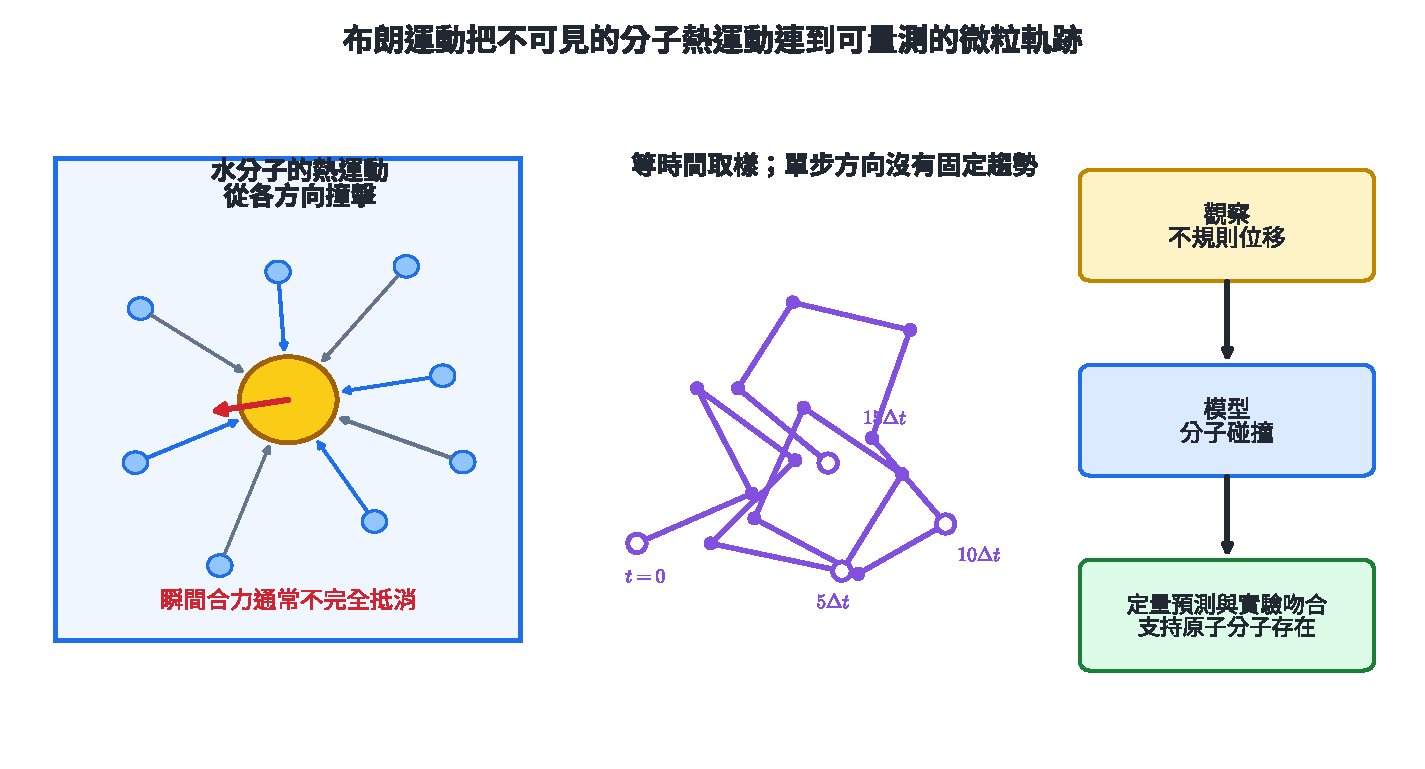
\includegraphics[keepaspectratio,alt={分子碰撞、等時間位置與布朗運動的證據鏈}]{assets/必物-2-原子存在的證據鏈.pdf}}
\caption{分子碰撞、等時間位置與布朗運動的證據鏈}
\end{figure}

這條證據鏈包含三個層次：

\begin{enumerate}
\def\labelenumi{\arabic{enumi}.}
\tightlist
\item
  觀察：懸浮微粒的位置隨時間呈不規則折線。
\item
  模型：周圍大量分子持續熱運動並造成不平衡撞擊。
\item
  定量檢驗：愛因斯坦由模型推導微粒運動與溫度、粒徑、液體性質及時間的關係；佩蘭的實驗結果與預測相符，也得到一致的亞佛加厥常數。
\end{enumerate}

掃描穿隧顯微鏡等工具可把原子尺度表面的量測訊號重建成影像，成為另一種證據。影像仍來自儀器與物理模型的轉換，因此可信結論同時依賴校正、重複量測與模型檢查。

布朗運動模型直接用於懸浮液、空氣微粒、藥物輸送、細胞內擴散及奈米粒子追蹤。粒徑愈小，分子碰撞造成的位置起伏通常愈容易觀察；溫度升高也會加強熱運動。

\subsubsection{示範 1　從觀察建立原子存在的證據鏈}\label{ux793aux7bc4-1-ux5f9eux89c0ux5bdfux5efaux7acbux539fux5b50ux5b58ux5728ux7684ux8b49ux64daux93c8}

顯微鏡每隔 \(1.0\ \mathrm s\) 記錄一顆懸浮微粒。軌跡不規則，而且把花粉換成無生命的煙塵後仍出現相似現象。判斷哪些敘述是觀察、模型與檢驗。

\begin{enumerate}
\def\labelenumi{\arabic{enumi}.}
\tightlist
\item
  「微粒每秒的位置不同，方向無固定規律」是直接觀察。
\item
  「微粒受到周圍水分子的不平衡撞擊」是微觀模型。
\item
  換成煙塵仍有相似運動，排除了「花粉本身具有生命才會動」的解釋。
\item
  若模型還能預測不同溫度、粒徑下的統計結果，並由實驗得到相符數值，證據強度會再提高。
\end{enumerate}

結論的重點是多項可重複的定量預測共同支持粒子模型。

\subsubsection{示範 2　由位移平方資料辨認布朗運動的統計規律}\label{ux793aux7bc4-2-ux7531ux4f4dux79fbux5e73ux65b9ux8cc7ux6599ux8fa8ux8a8dux5e03ux6717ux904bux52d5ux7684ux7d71ux8a08ux898fux5f8b}

某實驗在不同經過時間下，得到許多相同微粒的平均位移平方：

{\def\LTcaptype{none} % do not increment counter
\begin{longtable}[]{@{}rrrrr@{}}
\toprule\noalign{}
\(t\)（s） & 1.0 & 2.0 & 3.0 & 4.0 \\
\midrule\noalign{}
\endhead
\bottomrule\noalign{}
\endlastfoot
\(\langle r^2\rangle\)（\(\mu\mathrm m^2\)） & 2.1 & 4.0 & 6.2 & 8.1 \\
\end{longtable}
}

逐筆計算 \(\langle r^2\rangle/t\)：

\[
2.1,\ 2.0,\ 2.07,\ 2.03\ \mu\mathrm m^2/\mathrm s.
\]

比值近似固定，資料支持

\[
\langle r^2\rangle\propto t.
\]

這是群體統計規律；單一微粒的瞬時路徑仍可非常曲折。實驗用途是由軌跡資料反推擴散快慢或微粒尺寸。

\subsection{1.2 三態的粒子模型}\label{ux4e09ux614bux7684ux7c92ux5b50ux6a21ux578b}

物質狀態要在指定溫度與壓力下討論。同一物質改變溫度或壓力，粒子的平均動能、平均距離與束縛狀況會改變，因而可能發生熔化、汽化、凝結或凝固。

粒子間作用隨距離改變：

\begin{itemize}
\tightlist
\item
  距離太短時，電子雲強烈排斥，粒子難以繼續靠近。
\item
  在適當距離附近，吸引與排斥形成穩定間距。
\item
  距離很遠時，分子間作用迅速減弱；一般氣體模型常把它近似為可忽略。
\end{itemize}

\begin{figure}
\centering
\pandocbounded{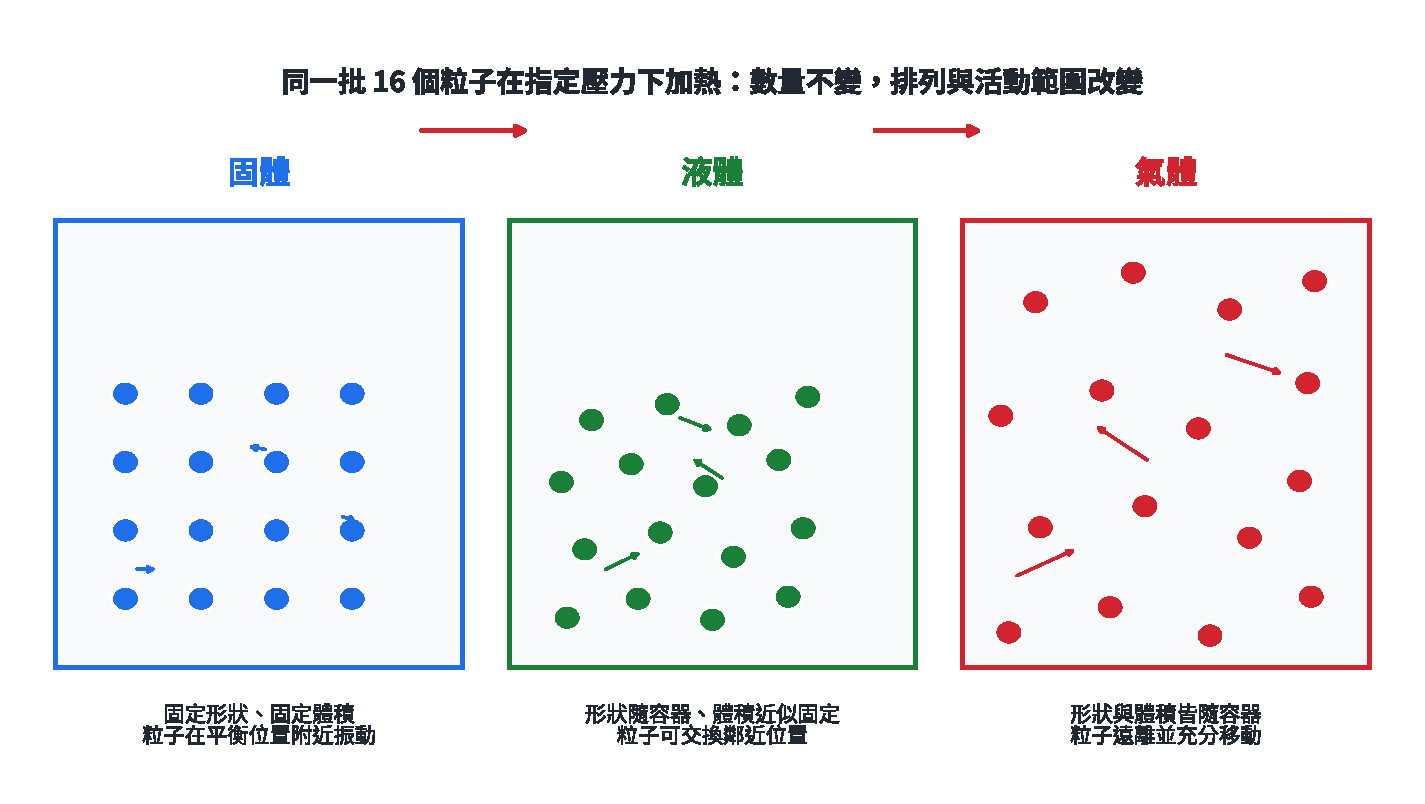
\includegraphics[keepaspectratio,alt={同一批粒子的三態排列、間距與運動}]{assets/必物-2-物質三態的粒子模型.pdf}}
\caption{同一批粒子的三態排列、間距與運動}
\end{figure}

由圖可推得三態的巨觀性質：

{\def\LTcaptype{none} % do not increment counter
\begin{longtable}[]{@{}llll@{}}
\toprule\noalign{}
狀態 & 微觀運動與束縛 & 形狀 & 體積 \\
\midrule\noalign{}
\endhead
\bottomrule\noalign{}
\endlastfoot
固體 & 粒子在平衡位置附近振動，鄰近關係大致維持 & 固定 & 固定 \\
液體 & 粒子仍相近，可交換鄰近位置並流動 & 隨容器 & 近似固定 \\
氣體 & 粒子平均距離大，可在容器內充分移動 & 隨容器 & 隨容器 \\
\end{longtable}
}

晶體中的粒子有規則排列；玻璃等非晶固體雖缺乏長程規則，粒子仍被限制在局部位置，因此也有固定形狀與體積。

粒子模型還能連到多種自然現象：

\begin{itemize}
\tightlist
\item
  聲音在空氣中傳播時，空氣粒子在平衡位置附近振動，把壓力變化傳給鄰近粒子。
\item
  湯匙的一端放入熱水後，粒子碰撞與金屬內電子傳遞能量，使較遠處升溫。
\item
  摩擦使電子在材料表面轉移，物體帶電後產生吸引或排斥。
\item
  太陽帶電粒子進入地球磁場附近並與大氣粒子碰撞，可使大氣原子或分子發光形成極光。
\end{itemize}

\subsubsection{示範 3　由微觀描述判斷物態}\label{ux793aux7bc4-3-ux7531ux5faeux89c0ux63cfux8ff0ux5224ux65b7ux7269ux614b}

某物質的粒子彼此相近，鄰近粒子會持續交換位置；把它倒入不同形狀的容器後，形狀改變而體積近似不變。

\begin{enumerate}
\def\labelenumi{\arabic{enumi}.}
\tightlist
\item
  粒子彼此相近，表示束縛仍足以維持平均距離。
\item
  鄰近粒子可交換位置，表示物質能流動。
\item
  形狀隨容器、體積近似固定，符合液體。
\end{enumerate}

因此這是液態。分類依據是粒子運動與巨觀形狀、體積的共同證據。

\subsubsection{示範 4　由加熱過程解釋固體熔化}\label{ux793aux7bc4-4-ux7531ux52a0ux71b1ux904eux7a0bux89e3ux91cbux56faux9ad4ux7194ux5316}

在固定外界壓力下加熱一塊固體：

\begin{enumerate}
\def\labelenumi{\arabic{enumi}.}
\tightlist
\item
  粒子平均動能增加，在平衡位置附近的振動幅度變大。
\item
  到達熔點附近，吸收的能量使原有排列與束縛被重新組織。
\item
  粒子開始能交換鄰近位置，材料取得流動性。
\item
  體積仍由粒子間吸引維持在有限範圍，所以液體保有近似固定體積。
\end{enumerate}

這項推理可用於選擇鑄造溫度、相變材料及低溫保存條件。

\subsection{1.3 節內練習}\label{ux7bc0ux5167ux7df4ux7fd2}

\begin{enumerate}
\def\labelenumi{\arabic{enumi}.}
\tightlist
\item
  說明元素、原子與分子三個概念的關係，並各舉一例。
\item
  布朗運動中，可見微粒的路徑不規則。寫出一項直接觀察、一項微觀模型與一項可增加模型可信度的後續檢驗。
\item
  同種微粒在 \(t=2.0,\ 4.0,\ 6.0\ \mathrm s\) 時的平均位移平方分別為 \(3.0,\ 6.1,\ 9.2\ \mu\mathrm m^2\)。判斷 \(\langle r^2\rangle\) 是否近似與 \(t\) 成正比。
\item
  比較固體、液體、氣體的粒子距離、運動自由度、形狀與體積。
\item
  在固定壓力下使液體冷卻並凝固。依粒子運動與束縛說明形狀為何由隨容器轉為固定。
\item
  分別用粒子交互作用說明：空氣傳聲、金屬湯匙導熱、塑膠尺摩擦後吸紙。
\end{enumerate}

\subsubsection{節內練習解析}\label{ux7bc0ux5167ux7df4ux7fd2ux89e3ux6790}

\begin{enumerate}
\def\labelenumi{\arabic{enumi}.}
\tightlist
\item
  元素由相同質子數定義，例如氧元素；原子是保有元素身分的粒子，例如 O；分子由原子鍵結，例如 \(\mathrm O_2\) 或 \(\mathrm H_2O\)。
\item
  觀察可寫微粒位置呈不規則折線；模型是周圍分子的熱運動造成不平衡碰撞；檢驗可改變溫度、粒徑或液體性質，再比較定量預測。
\item
  三個比值依序為 \(1.50,\ 1.525,\ 1.533\ \mu\mathrm m^2/\mathrm s\)，近似固定，因此資料支持成正比。
\item
  固體粒子相近且局部受限，固定形狀與體積；液體粒子相近但可交換位置，形狀隨容器、體積近似固定；氣體粒子平均距離大且充分移動，形狀與體積皆隨容器。
\item
  冷卻使平均動能下降；粒子逐漸被限制在局部平衡位置附近，鄰近關係固定，因而形成固定形狀。
\item
  傳聲靠粒子振動傳遞壓力變化；導熱靠粒子碰撞、晶格振動及金屬電子傳能；摩擦使電子轉移，帶異號電的材料產生靜電吸引。
\end{enumerate}

\section{2　原子的尺度與結構}\label{ux539fux5b50ux7684ux5c3aux5ea6ux8207ux7d50ux69cb}

\subsection{2.1 從原子到基本粒子的尺度}\label{ux5f9eux539fux5b50ux5230ux57faux672cux7c92ux5b50ux7684ux5c3aux5ea6}

常見原子的尺度約為

\[
10^{-10}\ \mathrm m=0.1\ \mathrm{nm}=1\ \text{Å}.
\]

不同原子大小略有差異，常見半徑約落在 \(0.03\) 至 \(0.3\ \mathrm{nm}\) 的量級。原子核尺度約為 \(10^{-15}\ \mathrm m\)，因此

\[
\frac{\text{原子尺度}}{\text{原子核尺度}}
\approx\frac{10^{-10}}{10^{-15}}=10^5.
\]

\begin{figure}
\centering
\pandocbounded{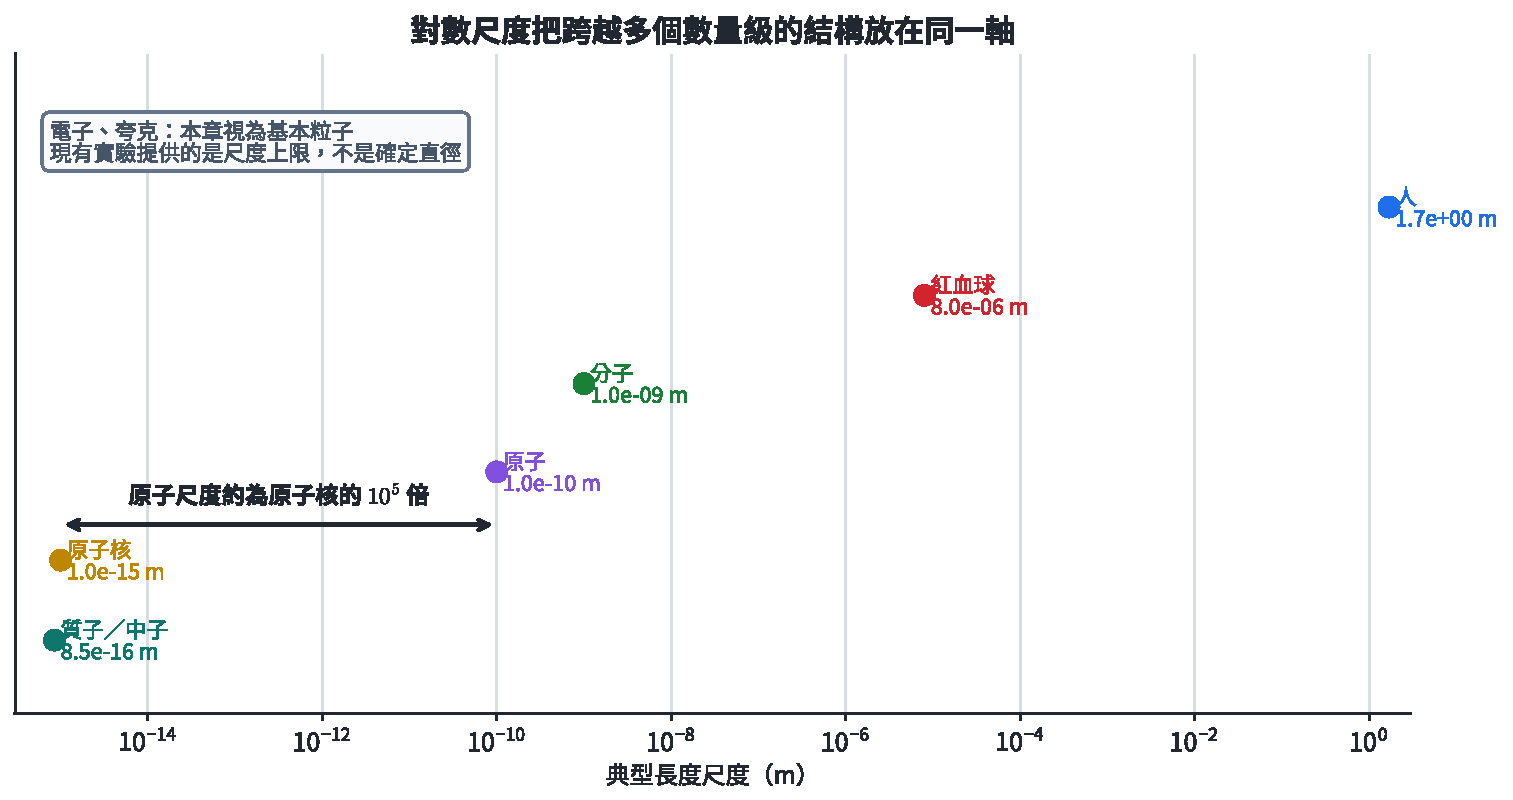
\includegraphics[keepaspectratio,alt={物質結構的對數尺度與基本粒子的量測限制}]{assets/必物-2-物質結構尺度階梯.pdf}}
\caption{物質結構的對數尺度與基本粒子的量測限制}
\end{figure}

若把直徑約 \(1\ \mathrm{fm}\) 的原子核放大成 \(1\ \mathrm{mm}\) 小球，保持比例的原子尺度約為

\[
(1\ \mathrm{mm})\times10^5=100\ \mathrm m.
\]

原子的大部分體積是電子分布的空間；原子的質量則幾乎集中於體積極小的原子核。尺度比例能幫助判斷顯微技術、散射探針與材料加工需要的解析度。

電子與夸克目前尚未觀察到內部結構，本章把它們視為基本粒子。質子與中子具有約 \(10^{-15}\ \mathrm m\) 的尺度，內部由夸克組成。

\subsubsection{示範 5　建立原子與原子核的比例模型}\label{ux793aux7bc4-5-ux5efaux7acbux539fux5b50ux8207ux539fux5b50ux6838ux7684ux6bd4ux4f8bux6a21ux578b}

把原子核畫成直徑 \(2.0\ \mathrm{mm}\) 的圓點，原子與原子核的尺度比取 \(10^5\)。求原子模型直徑。

\[
D_{\text{atom}}=(2.0\times10^{-3}\ \mathrm m)(10^5)
=2.0\times10^2\ \mathrm m.
\]

模型中的原子直徑為 \(200\ \mathrm m\)。這個比例顯示原子核雖承載幾乎全部質量，所占空間仍極小。

\subsubsection{示範 6　估計一條線上可排列多少個原子}\label{ux793aux7bc4-6-ux4f30ux8a08ux4e00ux689dux7ddaux4e0aux53efux6392ux5217ux591aux5c11ux500bux539fux5b50}

以原子間距 \(0.20\ \mathrm{nm}=2.0\times10^{-10}\ \mathrm m\) 估計，長度 \(1.0\ \mathrm{mm}\) 的直線可排列多少個原子？

\[
N\approx\frac{1.0\times10^{-3}}{2.0\times10^{-10}}
=5.0\times10^6.
\]

約有五百萬個。這種數量級估計可檢查奈米薄膜、晶格與半導體元件的尺度。

\subsection{2.2 散射實驗如何揭露原子核}\label{ux6563ux5c04ux5be6ux9a57ux5982ux4f55ux63edux9732ux539fux5b50ux6838}

湯姆森由氣體放電實驗發現各種原子都能釋出相同的帶負電粒子，即電子。他提出正電荷均勻分布於原子內、電子散布其中的模型。這個模型對高速、帶正電的 \(\alpha\) 粒子通過金箔作出預測：正電分散，單次作用很弱，粒子應大多近直線穿過，只出現小偏折。

拉塞福團隊讓 \(\alpha\) 粒子束撞擊極薄金箔，利用周圍閃爍屏記錄散射方向。

\begin{figure}
\centering
\pandocbounded{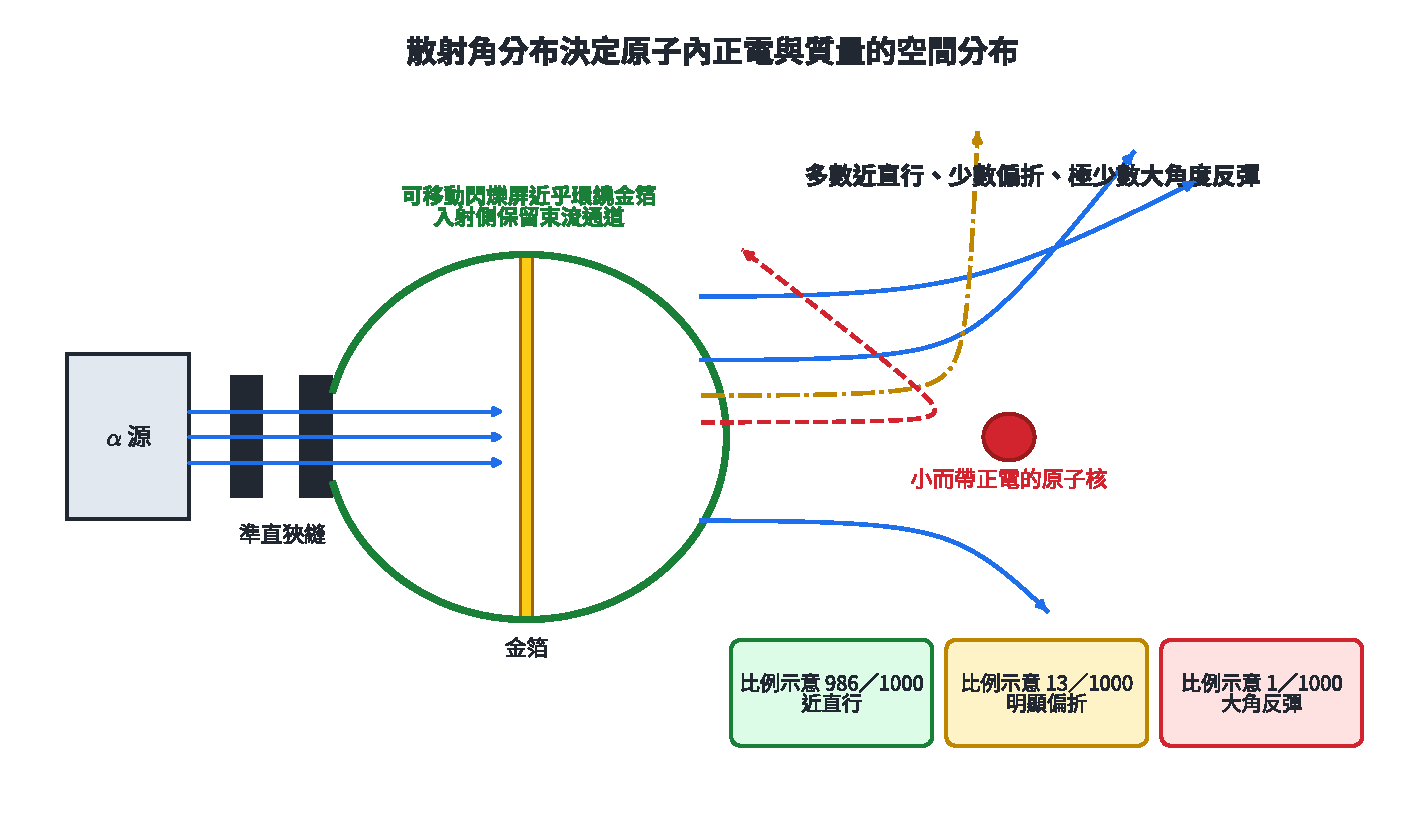
\includegraphics[keepaspectratio,alt={近乎環繞金箔的閃爍屏與拉塞福散射軌跡}]{assets/必物-2-拉塞福散射與原子核.pdf}}
\caption{近乎環繞金箔的閃爍屏與拉塞福散射軌跡}
\end{figure}

圖中的 1000 次是用來呈現「多數、少數、極少數」的比例示意。推理分成三步：

\begin{enumerate}
\def\labelenumi{\arabic{enumi}.}
\tightlist
\item
  絕大多數近直線通過：原子內大部分空間沒有集中物質阻擋。
\item
  少數明顯偏折：\(\alpha\) 粒子帶正電，附近存在集中的正電區域，靜電斥力能改變其方向。
\item
  極少數大角度反彈：能在很短距離產生巨大作用的正電荷與質量集中在很小體積內。
\end{enumerate}

因此拉塞福提出有核原子模型：原子核帶正電、質量幾乎集中於核內，核外是電子分布的空間。散射角愈大，通常代表粒子曾更接近原子核。

這種「已知探針射入樣品，量測出射方向與能量，再反推內部結構」的方法，也用於電子散射、粒子加速器、材料分析與醫療影像。

\subsubsection{示範 7　由散射資料選擇原子模型}\label{ux793aux7bc4-7-ux7531ux6563ux5c04ux8cc7ux6599ux9078ux64c7ux539fux5b50ux6a21ux578b}

某薄膜散射 20,000 顆帶正電探針，結果如下：

{\def\LTcaptype{none} % do not increment counter
\begin{longtable}[]{@{}lr@{}}
\toprule\noalign{}
結果 & 數目 \\
\midrule\noalign{}
\endhead
\bottomrule\noalign{}
\endlastfoot
偏折小於 \(5^\circ\) & 19,720 \\
偏折 \(5^\circ\) 至 \(90^\circ\) & 266 \\
偏折大於 \(90^\circ\) & 14 \\
\end{longtable}
}

\begin{enumerate}
\def\labelenumi{\arabic{enumi}.}
\tightlist
\item
  近直行比例為 \(19\,720/20\,000=98.6\%\)，表示樣品內大部分空間允許探針通過。
\item
  有 14 顆大角度反彈，表示少量探針遇到能造成強烈斥力的集中區。
\item
  探針與集中區同帶正電，因此偏折可由靜電斥力說明。
\end{enumerate}

資料支持「小而帶正電、承載大部分質量的原子核」，也說明單看平均偏折會漏掉關鍵的稀少事件。

\subsubsection{\texorpdfstring{示範 8　判斷 \(\alpha\) 粒子的受力與偏折方向}{示範 8　判斷 \textbackslash alpha 粒子的受力與偏折方向}}\label{ux793aux7bc4-8-ux5224ux65b7-alpha-ux7c92ux5b50ux7684ux53d7ux529bux8207ux504fux6298ux65b9ux5411}

一顆 \(\alpha\) 粒子由原子核上方從左向右射入。原子核與 \(\alpha\) 粒子都帶正電。

\begin{enumerate}
\def\labelenumi{\arabic{enumi}.}
\tightlist
\item
  靜電力沿兩者連線。
\item
  同號電荷互斥，所以原子核對 \(\alpha\) 粒子的力指向遠離原子核。
\item
  在核上方時，力具有向上分量，軌跡會向上彎。
\item
  最近距離愈小，庫侖力愈大，偏折角通常愈大。
\end{enumerate}

這個方向判斷先由圖上的相對位置與電性完成，再使用平方反比定律比較量值。

\subsection{2.3 原子核、核素與夸克}\label{ux539fux5b50ux6838ux6838ux7d20ux8207ux5938ux514b}

拉塞福由核反應辨認出帶正電、質量與氫核相近的質子。查兌克後來發現電中性、質量與質子相近的中子。原子由核外電子與原子核組成；原子核由質子與中子組成。最常見的氫核 \(^1_1\mathrm H\) 只有一個質子，氘核 \(^2_1\mathrm H\) 則另有一個中子。

{\def\LTcaptype{none} % do not increment counter
\begin{longtable}[]{@{}
  >{\raggedright\arraybackslash}p{(\linewidth - 8\tabcolsep) * \real{0.1667}}
  >{\raggedleft\arraybackslash}p{(\linewidth - 8\tabcolsep) * \real{0.2222}}
  >{\raggedleft\arraybackslash}p{(\linewidth - 8\tabcolsep) * \real{0.2222}}
  >{\raggedleft\arraybackslash}p{(\linewidth - 8\tabcolsep) * \real{0.2222}}
  >{\raggedright\arraybackslash}p{(\linewidth - 8\tabcolsep) * \real{0.1667}}@{}}
\toprule\noalign{}
\begin{minipage}[b]{\linewidth}\raggedright
粒子
\end{minipage} & \begin{minipage}[b]{\linewidth}\raggedleft
符號
\end{minipage} & \begin{minipage}[b]{\linewidth}\raggedleft
電荷
\end{minipage} & \begin{minipage}[b]{\linewidth}\raggedleft
靜止質量（約值）
\end{minipage} & \begin{minipage}[b]{\linewidth}\raggedright
位置
\end{minipage} \\
\midrule\noalign{}
\endhead
\bottomrule\noalign{}
\endlastfoot
電子 & \(e^-\) & \(-e=-1.602\times10^{-19}\ \mathrm C\) & \(9.11\times10^{-31}\ \mathrm{kg}\) & 核外 \\
質子 & \(p\) & \(+e\) & \(1.673\times10^{-27}\ \mathrm{kg}\) & 核內 \\
中子 & \(n\) & \(0\) & \(1.675\times10^{-27}\ \mathrm{kg}\) & 核內 \\
\end{longtable}
}

電子質量約為質子的 \(1/1836\)，所以原子質量幾乎由核子決定。

核素記號寫成

\[
{}^{A}_{Z}X^{z},
\]

其中：

\begin{itemize}
\tightlist
\item
  \(Z\) 是原子序，也是質子數。
\item
  \(A\) 是質量數，\(A=Z+N\)。
\item
  \(N=A-Z\) 是中子數。
\item
  \(z\) 是離子的帶電數；以 \(e\) 為單位時，電子數 \(N_e=Z-z\)。例如 \(z=+2\) 時少兩個電子，\(z=-1\) 時多一個電子。
\end{itemize}

同一元素的核素具有相同 \(Z\)、不同 \(N\)，稱為同位素。

\begin{figure}
\centering
\pandocbounded{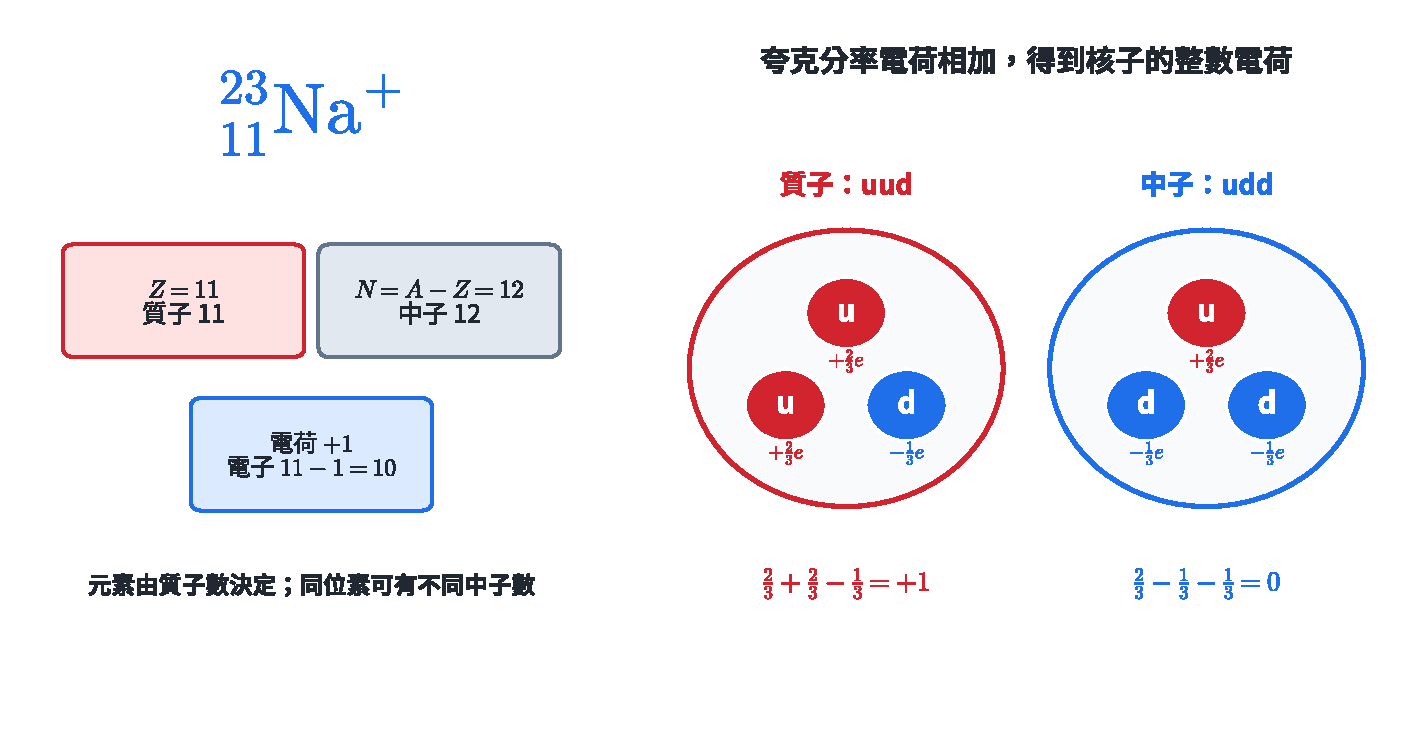
\includegraphics[keepaspectratio,alt={核素記號與夸克組成}]{assets/必物-2-核素記號與夸克組成.pdf}}
\caption{核素記號與夸克組成}
\end{figure}

質子和中子還能由上夸克 \(u\) 與下夸克 \(d\) 組成：

\[
q_u=+\frac{2}{3}e,\qquad q_d=-\frac{1}{3}e,
\]

\[
p=uud:\quad \frac{2}{3}e+\frac{2}{3}e-\frac{1}{3}e=+e,
\]

\[
n=udd:\quad \frac{2}{3}e-\frac{1}{3}e-\frac{1}{3}e=0.
\]

本章以 \(u,d\) 夸克說明普通物質中的質子與中子；其他夸克種類與希格斯粒子留待近代物理延伸。

\subsubsection{示範 9　由核素記號求三種粒子數}\label{ux793aux7bc4-9-ux7531ux6838ux7d20ux8a18ux865fux6c42ux4e09ux7a2eux7c92ux5b50ux6578}

求 \({}^{27}_{13}\mathrm{Al}^{3+}\) 的質子、中子與電子數。

\[
Z=13,\qquad N=A-Z=27-13=14.
\]

\(3+\) 表示少三個電子：

\[
N_e=13-3=10.
\]

所以質子 13 個、中子 14 個、電子 10 個。電荷檢查：

\[
13e-10e=+3e.
\]

\subsubsection{示範 10　由粒子數反推核素與離子}\label{ux793aux7bc4-10-ux7531ux7c92ux5b50ux6578ux53cdux63a8ux6838ux7d20ux8207ux96e2ux5b50}

某粒子含 17 個質子、18 個中子、18 個電子。

\begin{enumerate}
\def\labelenumi{\arabic{enumi}.}
\tightlist
\item
  \(Z=17\)，元素為氯 \(\mathrm{Cl}\)。
\item
  \(A=17+18=35\)。
\item
  電子比質子多 1 個，總電荷為 \(-e\)。
\end{enumerate}

核素與離子記號為

\[
{}^{35}_{17}\mathrm{Cl}^{-}.
\]

\subsubsection{示範 11　由電荷重建核子的夸克組成}\label{ux793aux7bc4-11-ux7531ux96fbux8377ux91cdux5efaux6838ux5b50ux7684ux5938ux514bux7d44ux6210}

三個夸克候選組合為 \(uuu\)、\(uud\)、\(udd\)。計算總電荷：

\[
uuu: 3\left(\frac{2}{3}e\right)=+2e,
\]

\[
uud: 2\left(\frac{2}{3}e\right)-\frac{1}{3}e=+e,
\]

\[
udd: \frac{2}{3}e-2\left(\frac{1}{3}e\right)=0.
\]

因此 \(uud\) 對應質子，\(udd\) 對應中子。這項檢查使用電荷守恆與分率電荷相加。

\subsection{2.4 節內練習}\label{ux7bc0ux5167ux7df4ux7fd2-1}

\begin{enumerate}
\def\labelenumi{\arabic{enumi}.}
\tightlist
\item
  將 \(0.25\ \mathrm{nm}\) 轉成公尺與埃，並判斷其是否屬於原子尺度。
\item
  原子核模型直徑為 \(0.50\ \mathrm{mm}\)，若原子與原子核尺度比為 \(10^5\)，求原子模型直徑。
\item
  依拉塞福散射結果，分別說明「大多數直行」與「極少數大角度反彈」支持的結構結論。
\item
  求 \({}^{56}_{26}\mathrm{Fe}^{2+}\) 的質子、中子與電子數。
\item
  某離子有 8 個質子、10 個中子、10 個電子，寫出核素與離子記號。
\item
  以夸克電荷驗證 \(uud\) 與 \(udd\) 的總電荷，並指出對應核子。
\end{enumerate}

\subsubsection{節內練習解析}\label{ux7bc0ux5167ux7df4ux7fd2ux89e3ux6790-1}

\begin{enumerate}
\def\labelenumi{\arabic{enumi}.}
\tightlist
\item
  \(0.25\ \mathrm{nm}=2.5\times10^{-10}\ \mathrm m=2.5\ \text{Å}\)，位於常見原子尺度。
\item
  \((0.50\times10^{-3})(10^5)=50\ \mathrm m\)。
\item
  大多數直行表示原子大部分是核外空間；大角度反彈表示正電荷與質量集中在極小原子核。
\item
  質子 \(26\)，中子 \(56-26=30\)，電子 \(26-2=24\)。
\item
  \(Z=8\) 為氧，\(A=8+10=18\)；電子比質子多 2 個，故為 \({}^{18}_{8}\mathrm O^{2-}\)。
\item
  \(uud\) 的電荷為 \(2(2/3)e-(1/3)e=+e\)，是質子；\(udd\) 的電荷為 \((2/3)e-2(1/3)e=0\)，是中子。
\end{enumerate}

\section{3　物質間的基本交互作用}\label{ux7269ux8ceaux9593ux7684ux57faux672cux4ea4ux4e92ux4f5cux7528}

交互作用描述兩個系統如何彼此改變。判斷一個現象時，可依序確認：

\begin{enumerate}
\def\labelenumi{\arabic{enumi}.}
\tightlist
\item
  作用的來源與承受作用的對象。
\item
  作用方向是吸引、排斥，或使粒子種類改變。
\item
  相關距離是天文、日常、原子核或更短尺度。
\item
  力量值如何隨質量、電量與距離改變。
\end{enumerate}

重力與電磁作用可跨長距離；強作用與弱作用集中在極短尺度。場是描述交互作用在空間中如何分布的物理量：先由來源建立場，再由置於場中的物體所受作用判定效果。

\subsection{3.1 萬有引力與重力場}\label{ux842cux6709ux5f15ux529bux8207ux91cdux529bux5834}

\begin{figure}
\centering
\pandocbounded{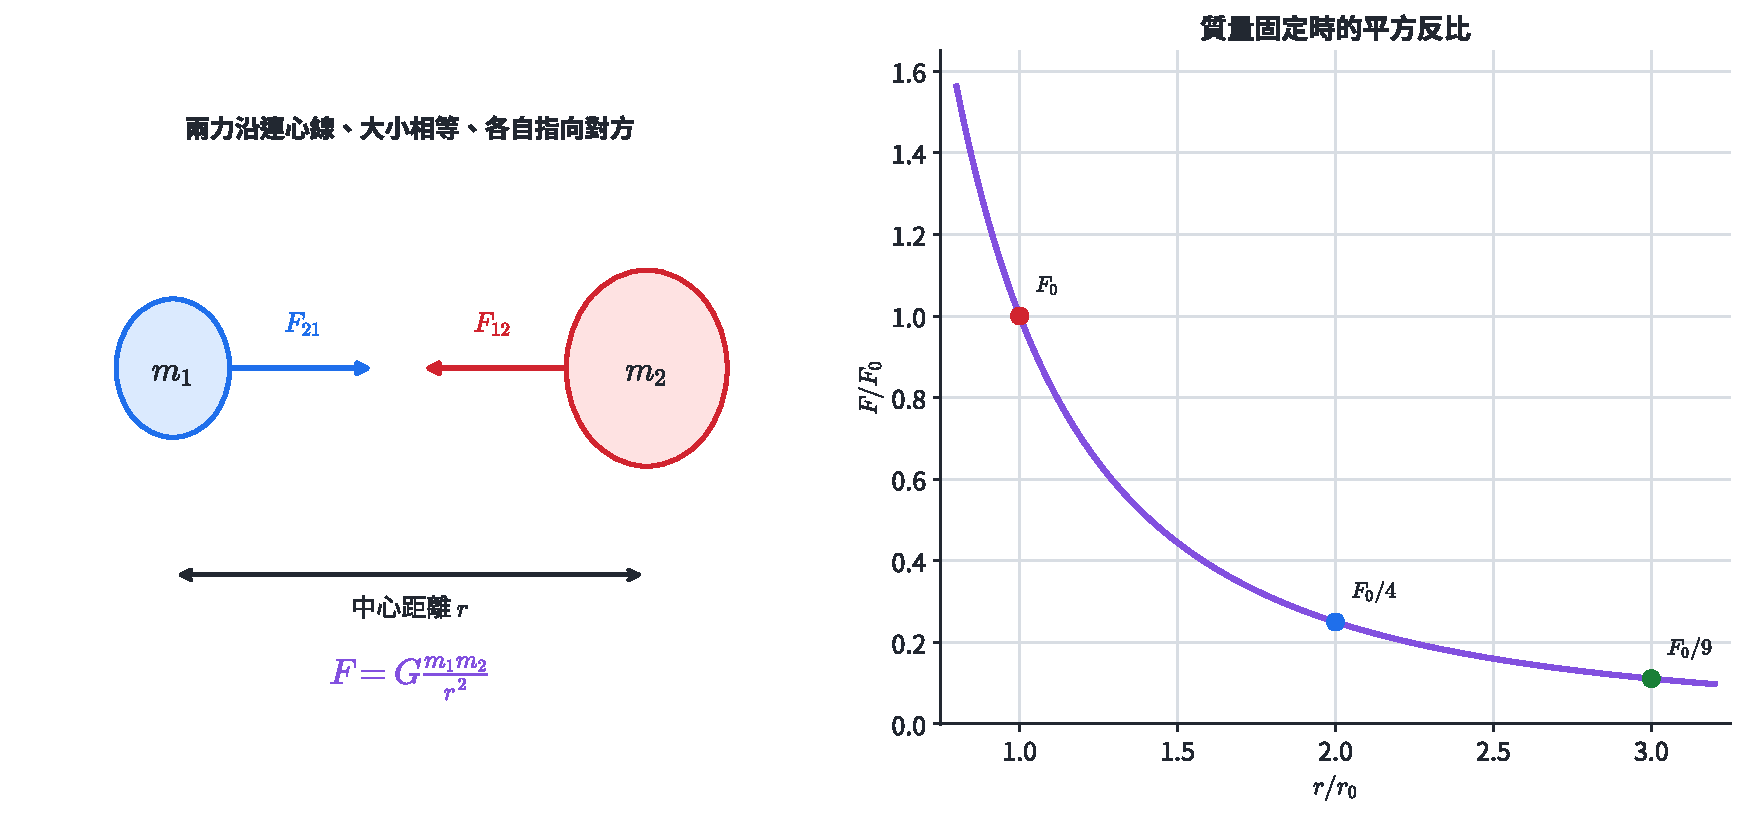
\includegraphics[keepaspectratio,alt={萬有引力與平方反比}]{assets/必物-2-萬有引力與平方反比.pdf}}
\caption{萬有引力與平方反比}
\end{figure}

質量為 \(m_1,m_2\) 的兩個質點，相距 \(r\) 時，萬有引力量值為

\[
F=G\frac{m_1m_2}{r^2},
\]

其中

\[
G=6.67\times10^{-11}\ \mathrm{N\,m^2/kg^2}.
\]

適用條件與方向：

\begin{itemize}
\tightlist
\item
  質點模型可直接使用；均勻球體的外部重力也可把質量視為集中於球心。
\item
  \(r\) 是兩質點或兩球心的距離。
\item
  兩力沿連心線，各自指向對方，量值相等。
\item
  質量固定時，距離變成 \(ar\)，力量值變成原來的 \(1/a^2\)。
\end{itemize}

質量 \(M\) 的球形天體，在距球心 \(r\) 處建立的重力場強度為

\[
g(r)=\frac{F}{m}=G\frac{M}{r^2}.
\]

它同時是放入小物體後的重力加速度。天體表面 \(r=R\)：

\[
g_{\text{surface}}=G\frac{M}{R^2},\qquad W=mg_{\text{surface}}.
\]

這個模型用於行星表面重量、衛星軌道、潮汐與天體質量估計。

\subsubsection{示範 12　同時改變質量與距離}\label{ux793aux7bc4-12-ux540cux6642ux6539ux8b8aux8ceaux91cfux8207ux8dddux96e2}

原本兩質量間的引力為 \(F\)。現在把 \(m_1\) 變為 \(2m_1\)、\(m_2\) 變為 \(3m_2\)，距離變為 \(2r\)。

先寫比值：

\[
\frac{F'}{F}
=\frac{(2m_1)(3m_2)}{m_1m_2}
\left(\frac{r}{2r}\right)^2
=6\cdot\frac{1}{4}=\frac{3}{2}.
\]

所以

\[
F'=1.5F.
\]

質量乘積提供 6 倍，距離平方提供 \(1/4\) 倍，兩項相乘得到結果。

\subsubsection{示範 13　比較星球表面重力加速度}\label{ux793aux7bc4-13-ux6bd4ux8f03ux661fux7403ux8868ux9762ux91cdux529bux52a0ux901fux5ea6}

某星球質量為地球的 \(8\) 倍，半徑為地球的 \(2\) 倍。以地表重力加速度 \(g_\oplus\) 為基準：

\[
\frac{g_{\text p}}{g_\oplus}
=\frac{8M_\oplus}{M_\oplus}
\left(\frac{R_\oplus}{2R_\oplus}\right)^2
=8\cdot\frac{1}{4}=2.
\]

所以 \(g_{\text p}=2g_\oplus\)。同一位太空人在該星球表面的重量為地球表面的 2 倍，質量則維持相同。

\clearpage

\subsection{3.2 電力、電場、磁力與磁場}\label{ux96fbux529bux96fbux5834ux78c1ux529bux8207ux78c1ux5834}

\subsubsection{點電荷與電場}\label{ux9edeux96fbux8377ux8207ux96fbux5834}

\begin{figure}
\centering
\pandocbounded{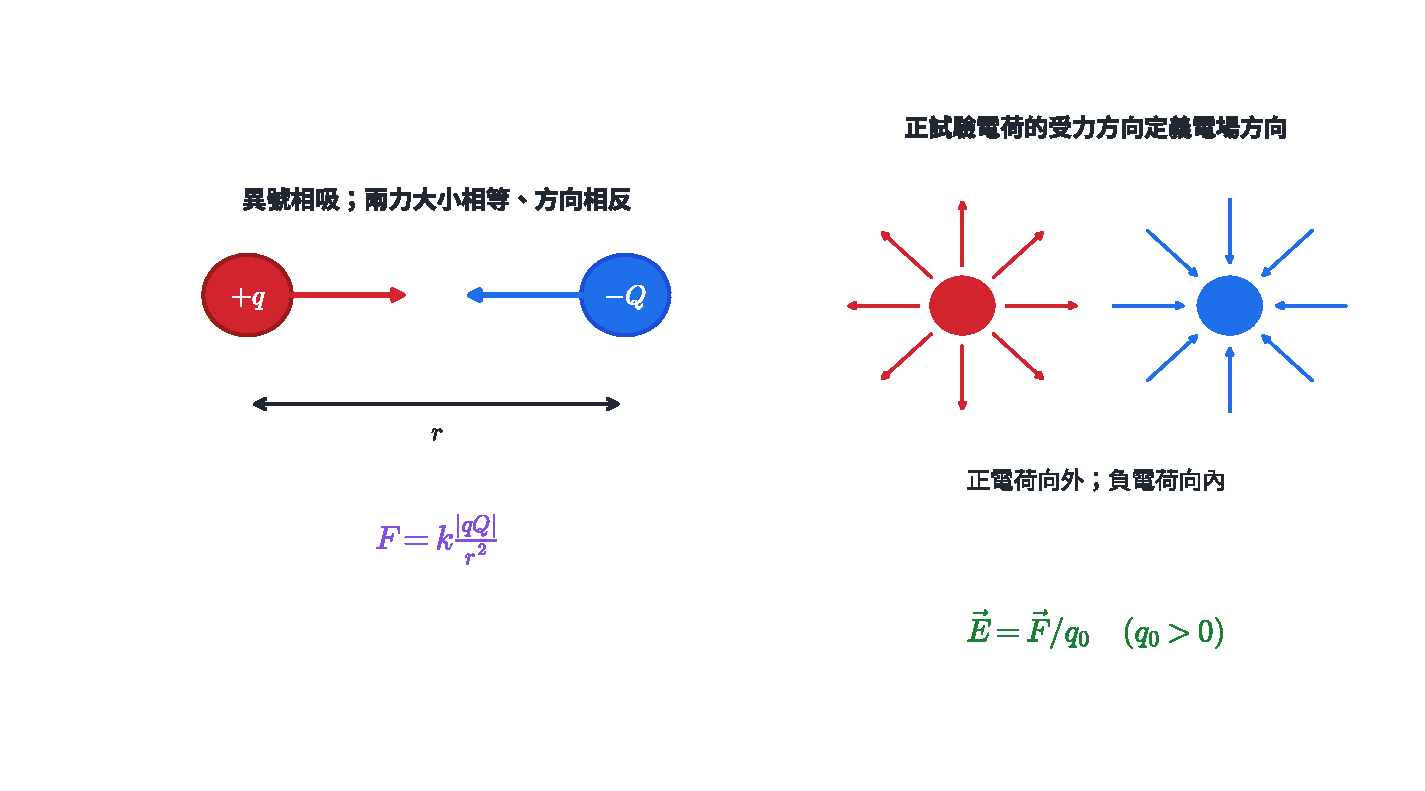
\includegraphics[keepaspectratio,alt={庫侖力與電場線}]{assets/必物-2-庫侖力與電場線.pdf}}
\caption{庫侖力與電場線}
\end{figure}

兩個近似靜止的點電荷 \(q_1,q_2\) 相距 \(r\)，庫侖力量值為

\[
F=k\frac{|q_1q_2|}{r^2},
\qquad
k=8.99\times10^9\ \mathrm{N\,m^2/C^2}.
\]

點電荷條件表示帶電體的大小遠小於彼此距離；均勻帶電球體的外部電場也可用球心點電荷模型。

\begin{itemize}
\tightlist
\item
  同號電荷互斥，異號電荷互吸。
\item
  兩力沿連心線，量值相等、方向相反。
\item
  電量乘積決定量值，距離平方決定衰減。
\end{itemize}

來源電荷在周圍建立電場。以小的正試驗電荷 \(q_0\) 定義某點電場：

\[
\vec E=\frac{\vec F}{q_0},\qquad q_0>0.
\]

點電荷 \(Q\) 的電場量值為

\[
E=k\frac{|Q|}{r^2}.
\]

正電荷場線向外，負電荷場線向內；任一點的場方向是場線切線方向。場線密處代表場較強。同一點的場方向唯一，所以場線彼此不相交。

帶電物體吸引另一物體時，來源可能是異號電荷，也可能是帶電體使中性導體內電荷重新分布而形成淨吸引。判斷電性時要再觀察排斥、接地或驗電器結果。

\subsubsection{磁極、磁化與磁場}\label{ux78c1ux6975ux78c1ux5316ux8207ux78c1ux5834}

\begin{figure}
\centering
\pandocbounded{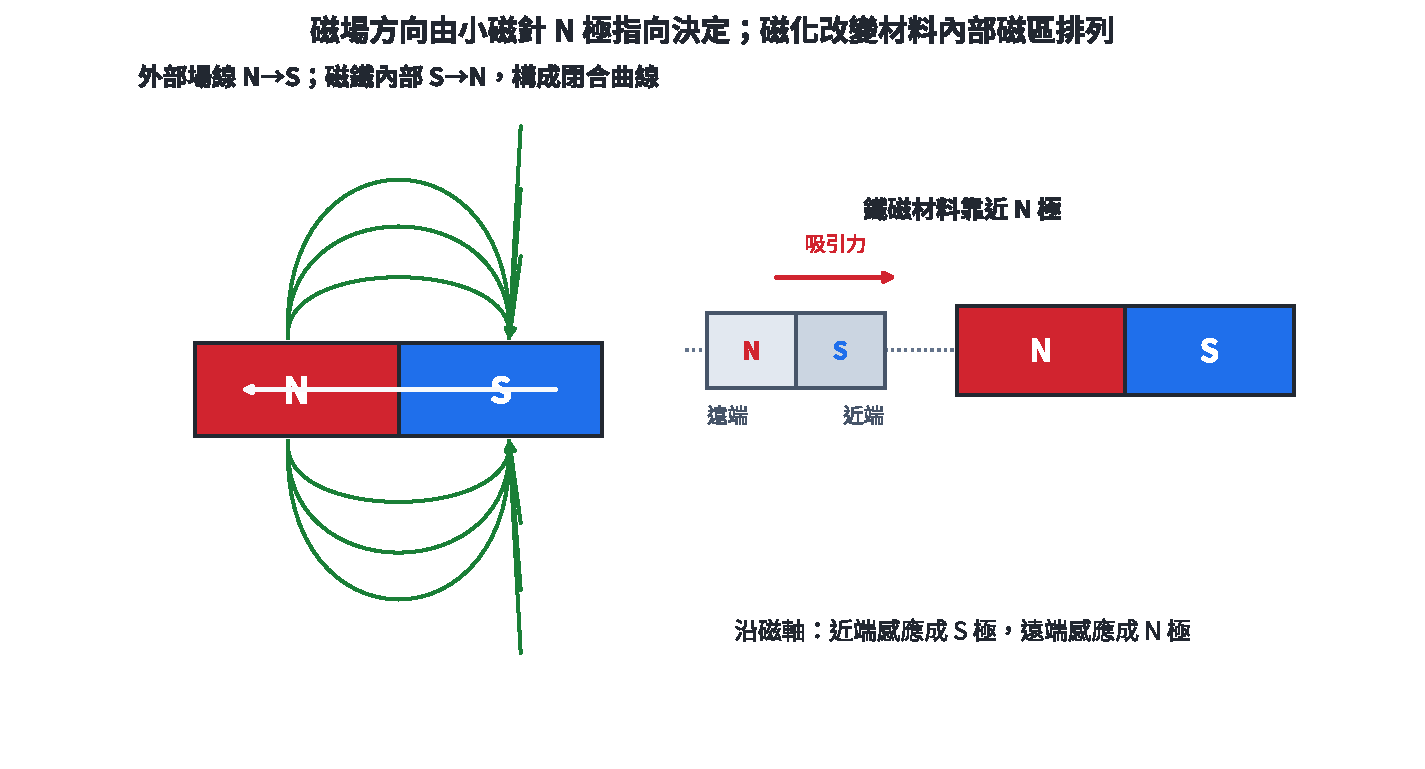
\includegraphics[keepaspectratio,alt={棒磁鐵閉合場線與鐵磁材料的近端、遠端磁化}]{assets/必物-2-磁場線與磁化.pdf}}
\caption{棒磁鐵閉合場線與鐵磁材料的近端、遠端磁化}
\end{figure}

棒磁鐵自由懸掛後，指北端定為 N 極，另一端為 S 極。同極相斥、異極相吸。切開一根磁鐵後，每一段都形成新的 N、S 兩極。

磁場方向定義為小磁針 N 極所指方向。棒磁鐵外部場線由 N 極指向 S 極，磁鐵內部由 S 極返回 N 極，構成閉合曲線；場線愈密處代表磁場愈強。

鐵、鈷、鎳及其部分合金可被磁化。鐵製物靠近磁鐵 N 極時，近端磁區傾向排列成 S 極，因此受到吸引。磁化解釋了磁鐵吸迴紋針，以及第一枚迴紋針再吸起下一枚的現象。

電力與磁力屬於同一種電磁作用。原子中的電子與原子核、原子間鍵結，以及日常的支撐力、彈性與摩擦，在本章層次都歸入電磁作用；更精確的材料微觀模型還會使用電子的量子性。

電場用於觸控面板、靜電除塵、影印與粒子束控制；磁場用於馬達、發電機、磁浮、資料儲存與醫療造影。

\subsubsection{示範 14　計算兩點電荷間的庫侖力}\label{ux793aux7bc4-14-ux8a08ux7b97ux5169ux9edeux96fbux8377ux9593ux7684ux5eabux4f96ux529b}

\(q_1=+2.0\ \mu\mathrm C\)、\(q_2=-3.0\ \mu\mathrm C\)，相距 \(0.30\ \mathrm m\)。

先由異號判斷為吸引。量值：

\[
F=(8.99\times10^9)
\frac{(2.0\times10^{-6})(3.0\times10^{-6})}{(0.30)^2}
=0.599\ \mathrm N
\approx0.60\ \mathrm N.
\]

作用在 \(q_1\) 上的力指向 \(q_2\)；作用在 \(q_2\) 上的力指向 \(q_1\)。兩力量值相同。

\subsubsection{示範 15　疊加兩個點電荷的電場}\label{ux793aux7bc4-15-ux758aux52a0ux5169ux500bux9edeux96fbux8377ux7684ux96fbux5834}

\(+4.0\ \mathrm{nC}\) 與 \(-4.0\ \mathrm{nC}\) 相距 \(0.40\ \mathrm m\)。求中點電場。

中點距每一電荷 \(0.20\ \mathrm m\)。

\begin{itemize}
\tightlist
\item
  正電荷的場在中點指向遠離正電荷，也就是指向負電荷。
\item
  負電荷的場在中點指向負電荷。
\end{itemize}

兩個方向相同，所以量值相加。每一個場為

\[
E_1=k\frac{|Q|}{r^2}
=(8.99\times10^9)\frac{4.0\times10^{-9}}{(0.20)^2}
=899\ \mathrm{N/C}.
\]

總電場

\[
E=2E_1=1.80\times10^3\ \mathrm{N/C},
\]

方向由正電荷指向負電荷。

\subsubsection{示範 16　判斷磁針與鐵片的方向}\label{ux793aux7bc4-16-ux5224ux65b7ux78c1ux91ddux8207ux9435ux7247ux7684ux65b9ux5411}

一小磁針放在棒磁鐵 S 極右側，另有一片未磁化鐵片放在 N 極左側。

\begin{enumerate}
\def\labelenumi{\arabic{enumi}.}
\tightlist
\item
  S 極右側的外部磁場指向 S 極，因此小磁針 N 極指向磁鐵。
\item
  鐵片靠近 N 極的一端感應成 S 極，遠端感應成 N 極。
\item
  近端距離較短，吸引效果較強，鐵片整體受到指向磁鐵的淨力。
\end{enumerate}

這項推理使用場方向、感應磁化與距離共同判斷。

\subsection{3.3 強作用與弱作用}\label{ux5f37ux4f5cux7528ux8207ux5f31ux4f5cux7528}

\begin{figure}
\centering
\pandocbounded{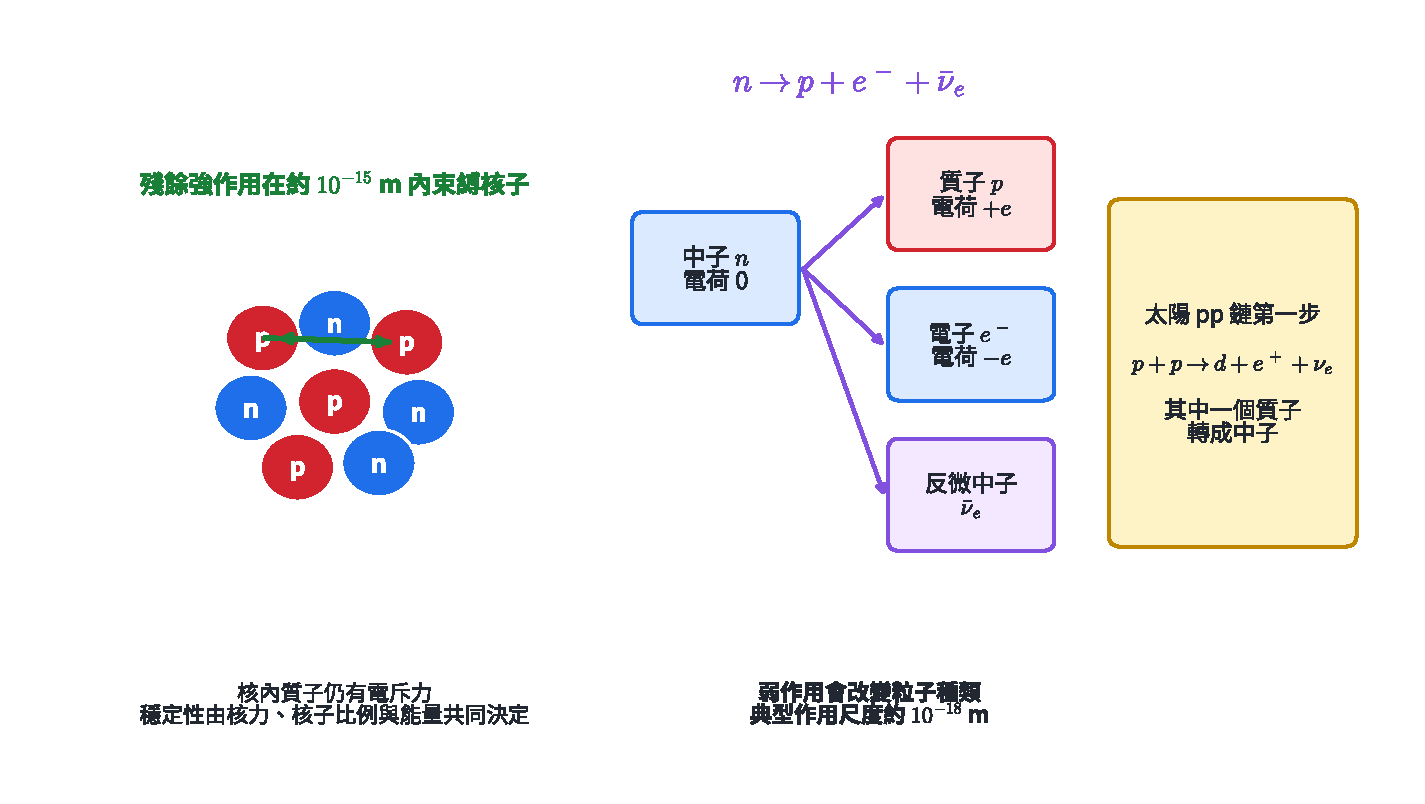
\includegraphics[keepaspectratio,alt={強作用與弱作用}]{assets/必物-2-強作用與弱作用.pdf}}
\caption{強作用與弱作用}
\end{figure}

強作用有兩個相關層次：

\begin{enumerate}
\def\labelenumi{\arabic{enumi}.}
\tightlist
\item
  夸克間的強作用把三個夸克束縛成質子或中子。
\item
  核子間的殘餘強作用在約 \(10^{-15}\ \mathrm m\) 尺度內吸引質子與中子，使許多原子核能穩定存在。
\end{enumerate}

核內質子彼此有靜電斥力。原子核的穩定由殘餘強作用、質子中子比例與核能量共同決定；核子距離超出核尺度後，殘餘強作用迅速減弱。

弱作用的特色是能使粒子種類改變。自由中子的 \(\beta^-\) 衰變可寫成

\[
n\rightarrow p+e^-+\bar{\nu}_e.
\]

電荷檢查：

\[
0=(+e)+(-e)+0.
\]

弱作用的典型尺度約為 \(10^{-18}\ \mathrm m\)。它參與原子核的 \(\beta\) 衰變，也參與太陽質子---質子鏈第一步：

\[
p+p\rightarrow d+e^++\nu_e,
\]

其中一個質子在反應中轉為中子，形成氘核 \(d\)。弱作用使太陽核融合的起始反應以穩定速率進行。

\subsubsection{示範 17　由反應特徵辨認強作用與弱作用}\label{ux793aux7bc4-17-ux7531ux53cdux61c9ux7279ux5fb5ux8fa8ux8a8dux5f37ux4f5cux7528ux8207ux5f31ux4f5cux7528}

判斷三個現象的主導作用：

\begin{enumerate}
\def\labelenumi{\arabic{enumi}.}
\tightlist
\item
  三個夸克形成質子：強作用。
\item
  質子與中子結合在原子核內：殘餘強作用。
\item
  中子轉成質子、電子與反微中子：弱作用，因為粒子種類發生轉換。
\end{enumerate}

辨認關鍵是「束縛夸克／核子」對應強作用，「\(\beta\) 衰變與種類轉換」對應弱作用。

\subsection{3.4 四種基本交互作用的比較}\label{ux56dbux7a2eux57faux672cux4ea4ux4e92ux4f5cux7528ux7684ux6bd4ux8f03}

\begin{figure}
\centering
\pandocbounded{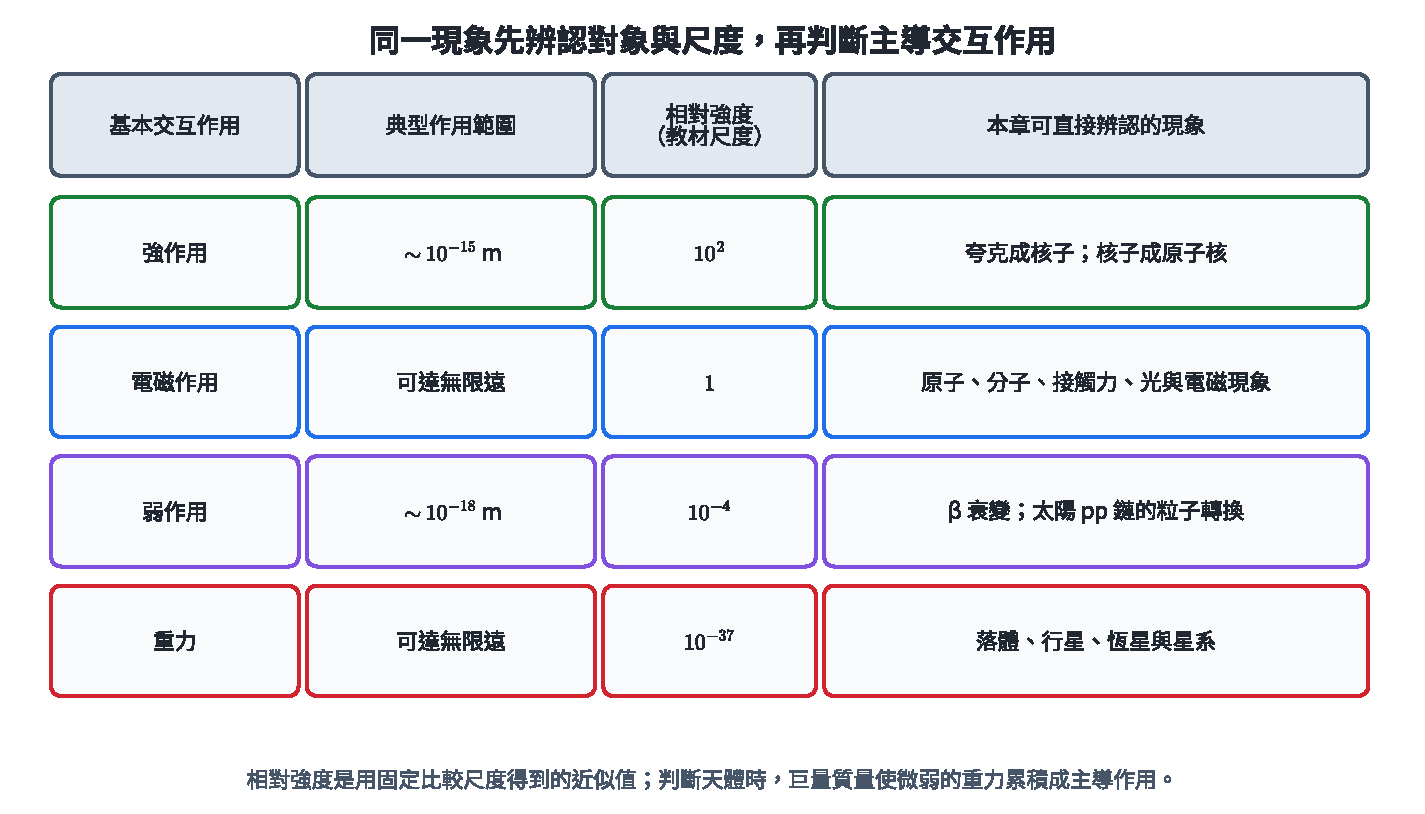
\includegraphics[keepaspectratio,alt={四種基本交互作用尺度圖}]{assets/必物-2-四種基本交互作用尺度圖.pdf}}
\caption{四種基本交互作用尺度圖}
\end{figure}

教材常用固定尺度下的約略相對強度比較四種作用：

{\def\LTcaptype{none} % do not increment counter
\begin{longtable}[]{@{}
  >{\raggedright\arraybackslash}p{(\linewidth - 6\tabcolsep) * \real{0.2143}}
  >{\raggedleft\arraybackslash}p{(\linewidth - 6\tabcolsep) * \real{0.2857}}
  >{\raggedleft\arraybackslash}p{(\linewidth - 6\tabcolsep) * \real{0.2857}}
  >{\raggedright\arraybackslash}p{(\linewidth - 6\tabcolsep) * \real{0.2143}}@{}}
\toprule\noalign{}
\begin{minipage}[b]{\linewidth}\raggedright
基本交互作用
\end{minipage} & \begin{minipage}[b]{\linewidth}\raggedleft
典型範圍
\end{minipage} & \begin{minipage}[b]{\linewidth}\raggedleft
約略相對強度
\end{minipage} & \begin{minipage}[b]{\linewidth}\raggedright
代表現象
\end{minipage} \\
\midrule\noalign{}
\endhead
\bottomrule\noalign{}
\endlastfoot
強作用 & 約 \(10^{-15}\ \mathrm m\) & \(10^2\) & 核子與原子核 \\
電磁作用 & 長程 & \(1\) & 原子、分子、接觸力、電與磁 \\
弱作用 & 約 \(10^{-18}\ \mathrm m\) & \(10^{-4}\) & \(\beta\) 衰變、太陽 pp 鏈 \\
重力 & 長程 & \(10^{-37}\) & 落體、行星、恆星與星系 \\
\end{longtable}
}

相對強度會隨比較尺度與過程改變，表中數值用於建立量級概念。重力對單一微觀粒子極弱，但天體質量巨大且重力只有吸引、可長程累積，因此在天文尺度主導。普通物質整體常接近電中性，使遠距離電力容易互相抵消；重力則隨質量持續累積。

\subsubsection{示範 18　由現象、對象與尺度選擇主導作用}\label{ux793aux7bc4-18-ux7531ux73feux8c61ux5c0dux8c61ux8207ux5c3aux5ea6ux9078ux64c7ux4e3bux5c0eux4f5cux7528}

{\def\LTcaptype{none} % do not increment counter
\begin{longtable}[]{@{}
  >{\raggedright\arraybackslash}p{(\linewidth - 4\tabcolsep) * \real{0.3333}}
  >{\raggedright\arraybackslash}p{(\linewidth - 4\tabcolsep) * \real{0.3333}}
  >{\raggedright\arraybackslash}p{(\linewidth - 4\tabcolsep) * \real{0.3333}}@{}}
\toprule\noalign{}
\begin{minipage}[b]{\linewidth}\raggedright
現象
\end{minipage} & \begin{minipage}[b]{\linewidth}\raggedright
判斷線索
\end{minipage} & \begin{minipage}[b]{\linewidth}\raggedright
主導作用
\end{minipage} \\
\midrule\noalign{}
\endhead
\bottomrule\noalign{}
\endlastfoot
月球繞地球 & 大質量、天文距離、吸引 & 重力 \\
電子受原子核吸引 & 帶異號電的粒子、原子尺度 & 電磁作用 \\
桌面支撐書本 & 原子電子雲接近形成接觸作用 & 電磁作用為主要來源 \\
質子與中子束縛成原子核 & 約 \(10^{-15}\ \mathrm m\)、核子束縛 & 殘餘強作用 \\
碳-14 發生 \(\beta^-\) 衰變 & 中子轉為質子並放出電子 & 弱作用 \\
\end{longtable}
}

同一系統可能同時含多種作用；題目通常要求找出決定主要觀測結果的作用。

\subsection{3.5 節內練習}\label{ux7bc0ux5167ux7df4ux7fd2-2}

\begin{enumerate}
\def\labelenumi{\arabic{enumi}.}
\tightlist
\item
  兩質點質量各變為原來的 2 倍，距離變為原來的 3 倍。求萬有引力與原值的比。
\item
  行星質量為地球的 \(4\) 倍、半徑為地球的 \(2\) 倍，求表面重力加速度與地球的比。
\item
  兩點電荷的其中一個電量變為 3 倍，距離變為原來的 \(\sqrt3\) 倍。求庫侖力與原值的比，並說明同號時方向。
\item
  說明棒磁鐵外部與內部場線方向；一枚鐵釘靠近 N 極時，近端感應成哪一極？
\item
  分別判斷「夸克形成質子」「核子形成原子核」「中子 \(\beta^-\) 衰變」的主導作用。
\item
  將下列現象分類到重力、電磁、強或弱作用：行星公轉、橡皮筋彈力、原子核束縛、太陽 pp 鏈起始反應。
\end{enumerate}

\subsubsection{節內練習解析}\label{ux7bc0ux5167ux7df4ux7fd2ux89e3ux6790-2}

\begin{enumerate}
\def\labelenumi{\arabic{enumi}.}
\tightlist
\item
  \(F'/F=(2)(2)/3^2=4/9\)。
\item
  \(g'/g=4/2^2=1\)，表面重力加速度相同。
\item
  \(F'/F=3/(\sqrt3)^2=1\)；同號時兩力沿連線、各自指離對方。
\item
  外部 N 至 S、內部 S 至 N，形成閉合曲線；鐵釘近端感應成 S 極。
\item
  依序為強作用、殘餘強作用、弱作用。
\item
  行星公轉---重力；橡皮筋彈力---以電磁作用為主要微觀來源；原子核束縛---殘餘強作用；pp 鏈起始粒子轉換---弱作用。
\end{enumerate}

\section{4　核心整理}\label{ux6838ux5fc3ux6574ux7406}

\subsection{物質與三態}\label{ux7269ux8ceaux8207ux4e09ux614b}

\begin{itemize}
\tightlist
\item
  布朗運動的可見不規則軌跡，可由不可見分子的熱運動與不平衡碰撞解釋；定量預測和實驗吻合支持原子分子模型。
\item
  固體粒子局部受限，液體粒子相近但可交換位置，氣體粒子平均距離大且充分移動。
\item
  聲、熱、靜電與極光都能由粒子運動和交互作用連到巨觀觀測。
\end{itemize}

\subsection{原子尺度與結構}\label{ux539fux5b50ux5c3aux5ea6ux8207ux7d50ux69cb}

\[
1\ \text{Å}=10^{-10}\ \mathrm m=0.1\ \mathrm{nm},
\qquad
\text{原子核尺度}\sim10^{-15}\ \mathrm m.
\]

\begin{itemize}
\tightlist
\item
  拉塞福散射：多數直行支持原子大部分為核外空間；少數大角偏折支持小而帶正電、承載大部分質量的原子核。
\item
  核素記號：\(A=Z+N\)；離子電子數由質子數與帶電數求得。
\item
  質子為 \(uud\)，電荷 \(+e\)；中子為 \(udd\)，電荷 0。
\end{itemize}

\subsection{四種基本交互作用}\label{ux56dbux7a2eux57faux672cux4ea4ux4e92ux4f5cux7528}

\[
F_{\mathrm g}=G\frac{m_1m_2}{r^2},
\qquad
F_{\mathrm e}=k\frac{|q_1q_2|}{r^2}.
\]

\begin{itemize}
\tightlist
\item
  重力長程且只有吸引，在天體尺度主導。
\item
  電磁作用有吸引與排斥，維繫原子、分子，也形成多數日常接觸作用。
\item
  強作用束縛夸克；殘餘強作用束縛核子。
\item
  弱作用造成 \(\beta\) 衰變等粒子種類轉換。
\end{itemize}

\section{5　章末代表題：分層與跨節整合}\label{ux7ae0ux672bux4ee3ux8868ux984cux5206ux5c64ux8207ux8de8ux7bc0ux6574ux5408}

第 1--4 題處理物質組成與三態，第 5--8 題處理尺度、散射、核素與夸克，第 9--12 題處理四種基本交互作用，第 13--16 題整合兩個以上主節。

\subsection{題目}\label{ux984cux76ee}

\begin{enumerate}
\def\labelenumi{\arabic{enumi}.}
\item
  道耳頓原子說、布朗運動、愛因斯坦模型與佩蘭實驗在原子論發展中各扮演什麼角色？
\item
  某懸浮微粒的平均位移平方資料如下：

  {\def\LTcaptype{none} % do not increment counter
  \begin{longtable}[]{@{}rrrrr@{}}
  \toprule\noalign{}
  \(t\)（s） & 1 & 2 & 4 & 8 \\
  \midrule\noalign{}
  \endhead
  \bottomrule\noalign{}
  \endlastfoot
  \(\langle r^2\rangle\)（\(\mu\mathrm m^2\)） & 1.8 & 3.7 & 7.3 & 14.6 \\
  \end{longtable}
  }

  判斷資料支持哪一項時間關係，並說明單一微粒軌跡與統計規律的差異。
\item
  一種物質具有固定體積，倒入細長容器與寬容器時形狀會改變。由微觀粒子模型判斷物態，並說明加熱至汽化後形狀、體積與粒子距離如何改變。
\item
  分別以粒子模型說明：（甲）空氣傳遞聲音；（乙）鐵湯匙由一端逐步升溫；（丙）塑膠尺摩擦紙後吸引紙屑。
\item
  原子尺度取 \(1.0\times10^{-10}\ \mathrm m\)、原子核尺度取 \(1.0\times10^{-15}\ \mathrm m\)。若把原子核放大成直徑 \(5.0\ \mathrm{mm}\)，原子模型直徑是多少？
\item
  金箔散射中，99\% 以上的 \(\alpha\) 粒子近直線通過，少量粒子偏折，極少量大角度反彈。依序寫出三項觀測對原子結構的推論。
\item
  求 \({}^{40}_{20}\mathrm{Ca}^{2+}\) 的質子、中子、電子數。另一粒子有 20 個質子、22 個中子、18 個電子，寫出其核素與離子記號，並判斷兩者是否為同位素。
\item
  已知 \(u\) 夸克電荷為 \(+2e/3\)、\(d\) 夸克為 \(-e/3\)。計算 \(uud\)、\(udd\)、\(uuu\) 的總電荷，指出質子與中子。
\item
  兩顆衛星質量分別為 \(m\) 與 \(2m\)，中心距離為 \(r\)，引力為 \(F\)。若第二顆衛星質量變為 \(6m\)，中心距離變為 \(3r\)，新引力是多少？
\item
  某星球質量為地球的 \(9\) 倍，半徑為地球的 \(3\) 倍。求星球表面重力加速度與地球的比，並比較同一物體在兩處的質量與重量。
\item
  \(+Q\) 與 \(-Q\) 相距 \(2a\)。判斷中點電場方向；若 \(Q\) 變為 2 倍、\(a\) 變為 2 倍，中點電場量值變為原來多少倍？
\item
  說明下列現象的主導交互作用：（甲）棒磁鐵吸起迴紋針；（乙）核子束縛成原子核；（丙）自由中子 \(\beta^-\) 衰變；（丁）地球繞太陽。
\item
  奈米粒子直徑為 \(80\ \mathrm{nm}\)，懸浮於水中並出現布朗運動。
\end{enumerate}

（1）粒子直徑約為 \(0.20\ \mathrm{nm}\) 原子尺度的多少倍？

（2）寫出支持「水由持續熱運動的分子組成」的觀察、模型與一項可控制的實驗變因。

（3）若水凝固，水分子的運動方式與材料的形狀如何改變？

\begin{enumerate}
\def\labelenumi{\arabic{enumi}.}
\setcounter{enumi}{13}
\tightlist
\item
  帶 \(+2e\) 的 \(\alpha\) 粒子從帶正電原子核上方通過，最近距離由 \(r\) 降為 \(r/2\)。
\end{enumerate}

（1）畫出原子核對 \(\alpha\) 粒子的受力方向。

（2）在點電荷近似下，最近點庫侖力變為原來多少倍？

（3）預測偏折角如何改變，並連結到拉塞福對原子核的推論。

\begin{enumerate}
\def\labelenumi{\arabic{enumi}.}
\setcounter{enumi}{14}
\tightlist
\item
  一顆球形星球質量 \(4M_\oplus\)、半徑 \(2R_\oplus\)。星球表面有質量 \(1.0\times10^{-9}\ \mathrm{kg}\)、電量 \(+2.0\times10^{-9}\ \mathrm C\) 的帶電微粒；上方電極在微粒處產生向上 \(5.0\ \mathrm{N/C}\) 的電場。取 \(g_\oplus=9.8\ \mathrm{m/s^2}\)。
\end{enumerate}

（1）求星球表面 \(g\)。

（2）求微粒所受重力與電力的量值及方向。

（3）判斷哪一作用較大，並指出兩力分別屬於哪種基本交互作用。

\begin{enumerate}
\def\labelenumi{\arabic{enumi}.}
\setcounter{enumi}{15}
\tightlist
\item
  碳-14 發生
\end{enumerate}

\[
{}^{14}_{6}\mathrm C\rightarrow{}^{14}_{7}\mathrm N+e^-+\bar\nu_e.
\]

（1）求衰變前後兩個原子核的質子與中子數。

（2）檢查反應兩側電荷。

（3）指出造成粒子轉換、束縛核子、束縛核外電子的三種作用。

（4）說明這個反應如何同時連結核素記號、粒子結構與基本交互作用。

\clearpage

\section{6　章末詳解}\label{ux7ae0ux672bux8a73ux89e3}

\subsection{第 1 題}\label{ux7b2c-1-ux984c}

\begin{figure}
\centering
\pandocbounded{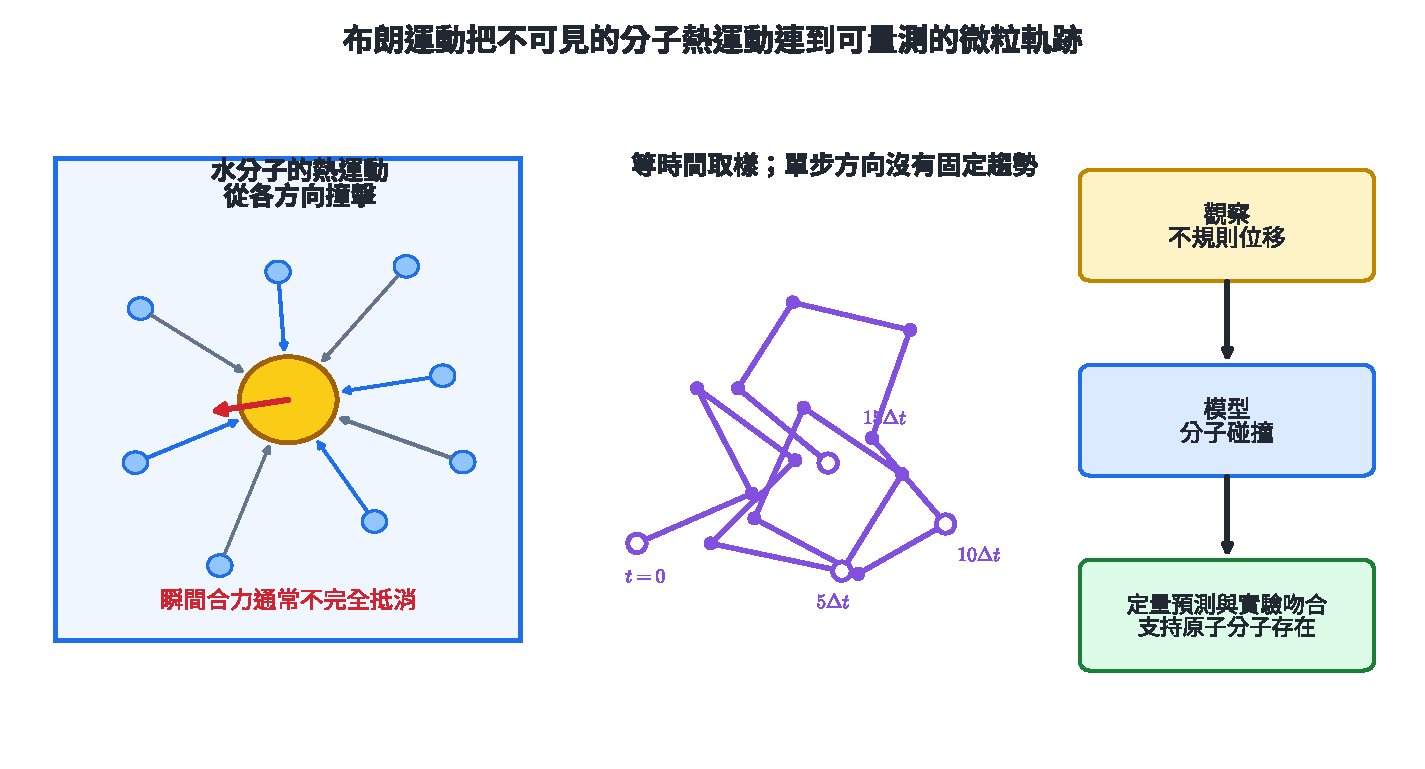
\includegraphics[keepaspectratio,alt={分子碰撞、等時間位置與布朗運動的證據鏈}]{assets/必物-2-原子存在的證據鏈.pdf}}
\caption{分子碰撞、等時間位置與布朗運動的證據鏈}
\end{figure}

道耳頓用原子假說統整元素與化學反應中的質量關係，提供可計算模型。布朗觀察到懸浮微粒持續不規則移動，提供待解釋的現象。愛因斯坦用分子熱運動與碰撞建立定量模型，導出可測預測。佩蘭實驗得到與預測相符的統計結果與亞佛加厥常數，使原子分子模型獲得獨立支持。

推理鏈為

\[
\text{化學規律}
\rightarrow\text{原子假說}
\rightarrow\text{布朗運動}
\rightarrow\text{分子碰撞模型}
\rightarrow\text{定量實驗吻合}.
\]

\subsection{第 2 題}\label{ux7b2c-2-ux984c}

計算比值：

\[
\frac{\langle r^2\rangle}{t}
=1.8,\ 1.85,\ 1.825,\ 1.825\ \mu\mathrm m^2/\mathrm s.
\]

比值近似固定，所以資料支持

\[
\langle r^2\rangle\propto t.
\]

單一微粒每一步方向隨機，軌跡呈曲折折線；大量同條件微粒的平均位移平方則呈穩定的時間比例。模型比較要用統計量，不以單一路徑要求平滑。

\subsection{第 3 題}\label{ux7b2c-3-ux984c}

\begin{figure}
\centering
\pandocbounded{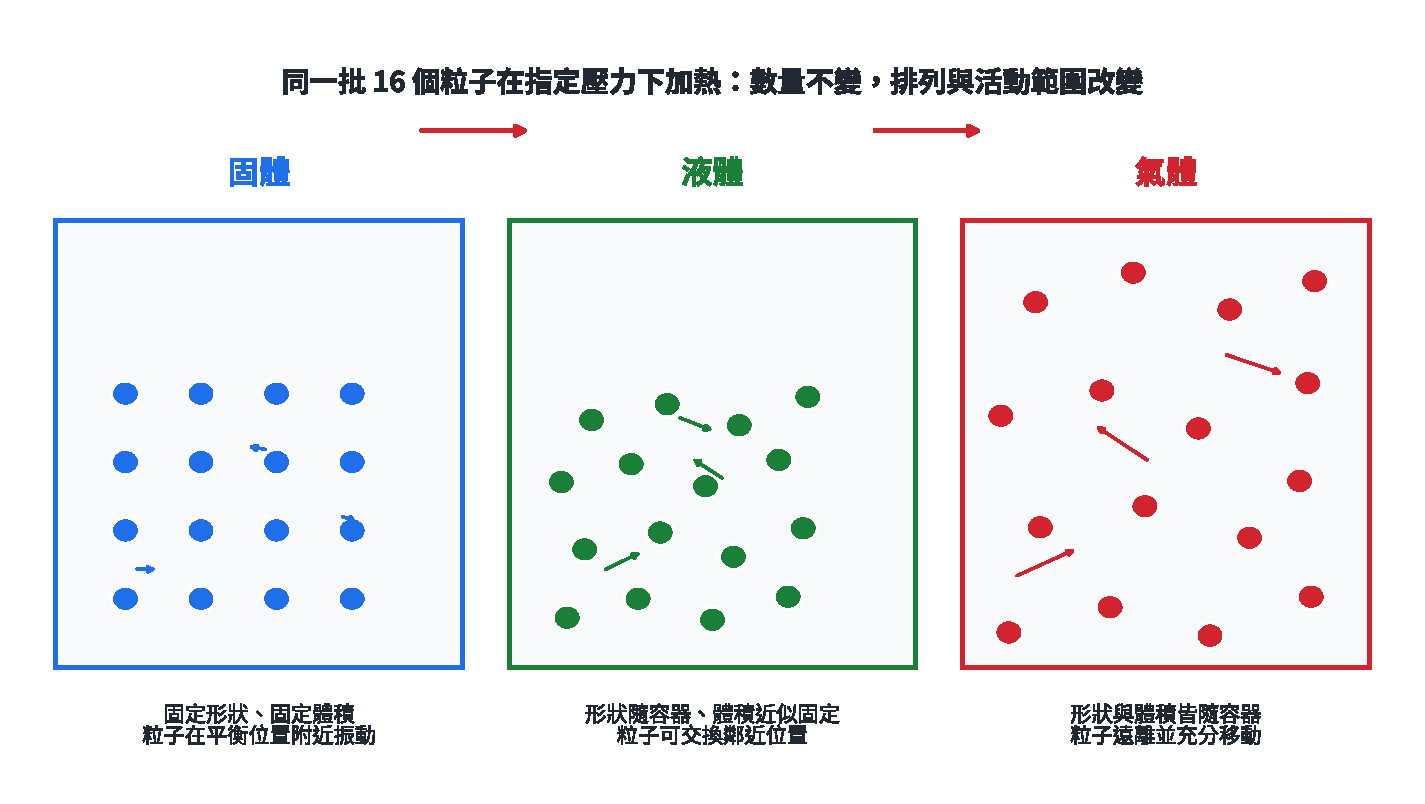
\includegraphics[keepaspectratio,alt={同一批粒子的三態排列、間距與運動}]{assets/必物-2-物質三態的粒子模型.pdf}}
\caption{同一批粒子的三態排列、間距與運動}
\end{figure}

固定體積、形狀隨容器，判斷為液體。液體粒子彼此相近，吸引仍能維持有限平均距離，但粒子可交換鄰近位置，因此能流動。

汽化後：

\begin{itemize}
\tightlist
\item
  粒子平均距離大幅增加。
\item
  粒子在容器中充分移動。
\item
  形狀隨容器。
\item
  體積也隨容器並容易壓縮。
\end{itemize}

模型條件是比較同一物質在指定外界壓力下的狀態改變。

\subsection{第 4 題}\label{ux7b2c-4-ux984c}

甲：聲源使鄰近空氣粒子振動，粒子把壓力變化傳給下一層，能量向外傳遞，空氣整體沒有隨聲波一路前進。

乙：熱水端的粒子與金屬內粒子碰撞；晶格振動與金屬電子逐步把能量傳向較冷端。

丙：摩擦使電子在材料表面轉移，塑膠尺與紙形成電荷分布；異號電荷或感應電荷分布造成淨吸引。三者都由微觀粒子運動與交互作用連到巨觀結果。

\subsection{第 5 題}\label{ux7b2c-5-ux984c}

\begin{figure}
\centering
\pandocbounded{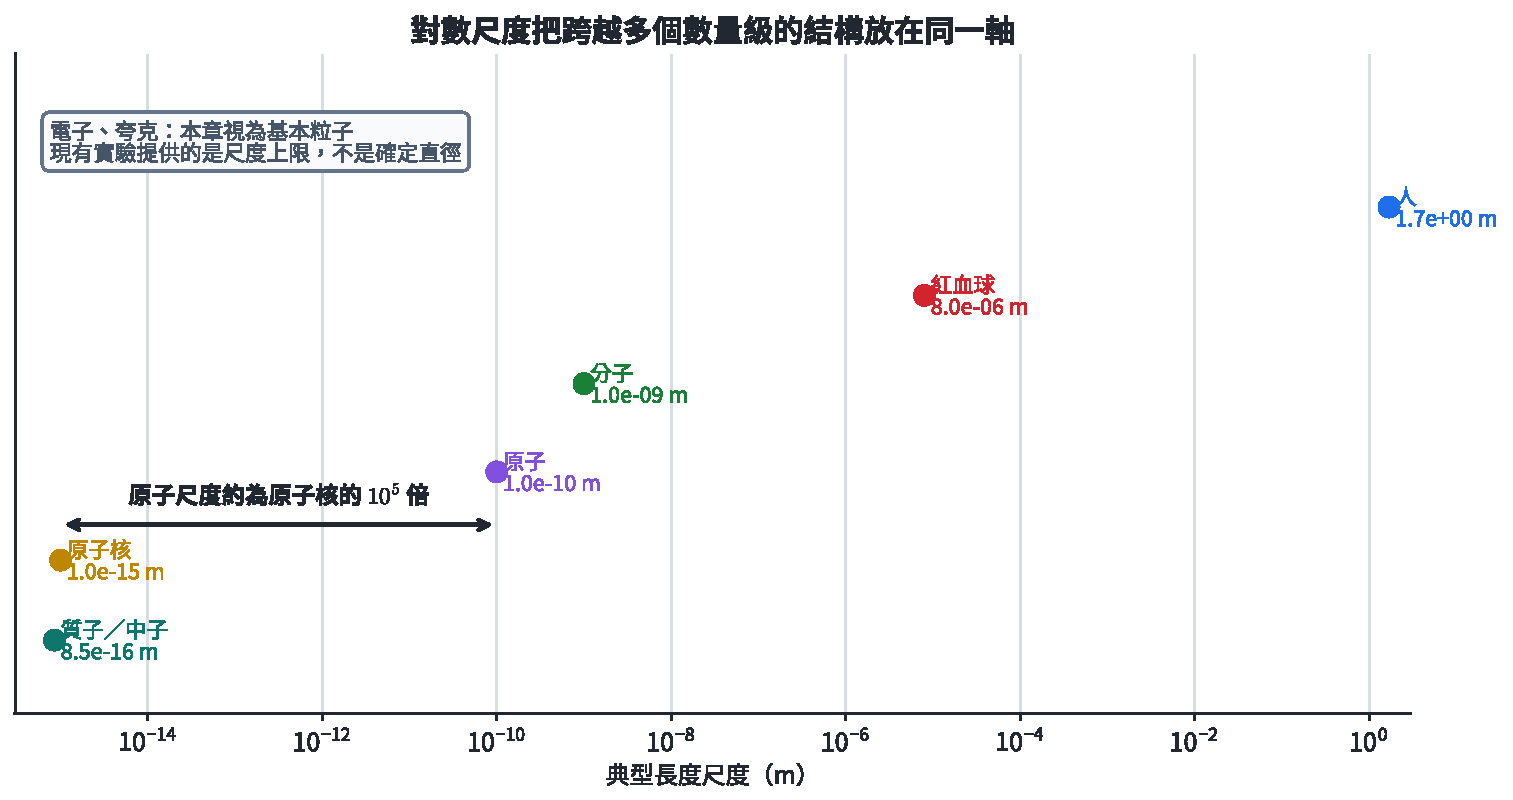
\includegraphics[keepaspectratio,alt={物質結構的對數尺度與基本粒子的量測限制}]{assets/必物-2-物質結構尺度階梯.pdf}}
\caption{物質結構的對數尺度與基本粒子的量測限制}
\end{figure}

尺度比：

\[
\frac{10^{-10}}{10^{-15}}=10^5.
\]

放大後原子直徑：

\[
D=(5.0\times10^{-3}\ \mathrm m)(10^5)
=5.0\times10^2\ \mathrm m.
\]

答案為 \(500\ \mathrm m\)。原子核占原子線尺度的十萬分之一。

\subsection{第 6 題}\label{ux7b2c-6-ux984c}

\begin{figure}
\centering
\pandocbounded{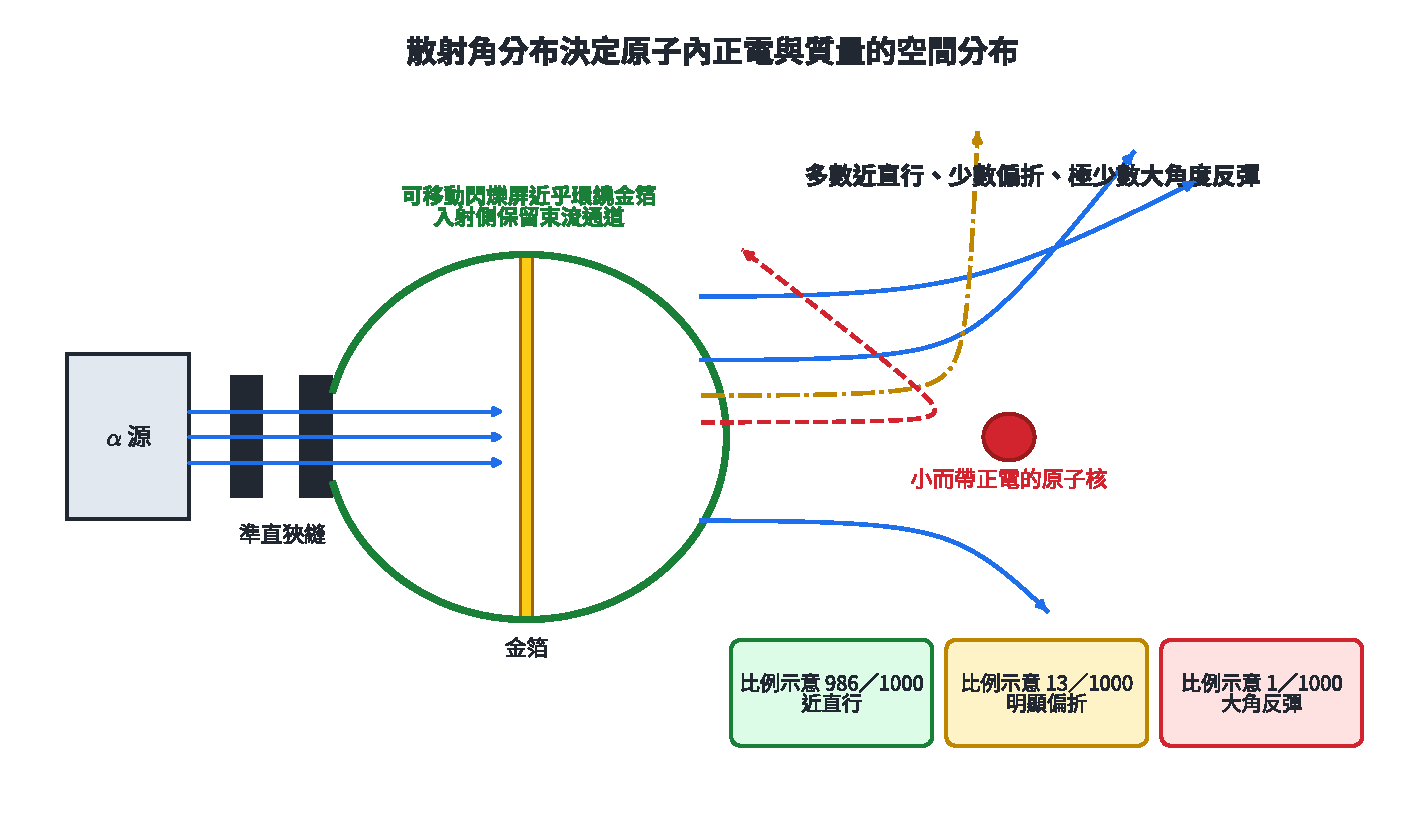
\includegraphics[keepaspectratio,alt={近乎環繞金箔的閃爍屏與拉塞福散射軌跡}]{assets/必物-2-拉塞福散射與原子核.pdf}}
\caption{近乎環繞金箔的閃爍屏與拉塞福散射軌跡}
\end{figure}

\begin{enumerate}
\def\labelenumi{\arabic{enumi}.}
\tightlist
\item
  多數近直行：原子內大部分體積是核外空間。
\item
  少量偏折：原子內存在集中正電區，對正電 \(\alpha\) 粒子施斥力。
\item
  極少量大角反彈：正電荷與幾乎全部質量集中於非常小的原子核。
\end{enumerate}

三項觀測要合併解釋；只有「多數直行」還無法單獨確定集中正電核的性質。

\subsection{第 7 題}\label{ux7b2c-7-ux984c}

\begin{figure}
\centering
\pandocbounded{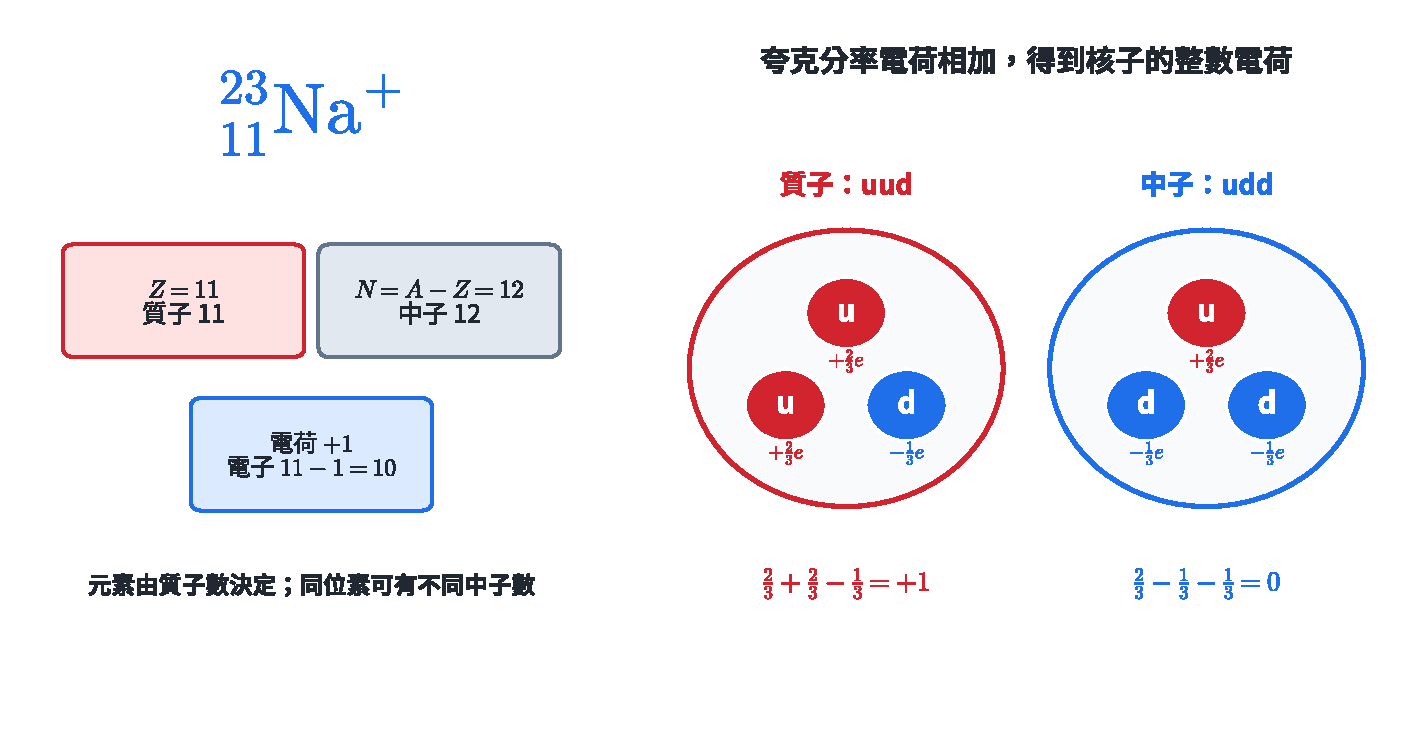
\includegraphics[keepaspectratio,alt={核素記號與夸克組成}]{assets/必物-2-核素記號與夸克組成.pdf}}
\caption{核素記號與夸克組成}
\end{figure}

對 \({}^{40}_{20}\mathrm{Ca}^{2+}\)：

\[
p=20,\qquad n=40-20=20,\qquad e=20-2=18.
\]

另一粒子：

\[
Z=20,\qquad A=20+22=42,
\]

且 18 個電子表示電荷為 \(+2e\)，所以記為

\[
{}^{42}_{20}\mathrm{Ca}^{2+}.
\]

兩者 \(Z\) 都是 20，中子數分別 20 與 22，因此是鈣的同位素。

\subsection{第 8 題}\label{ux7b2c-8-ux984c}

\begin{figure}
\centering
\pandocbounded{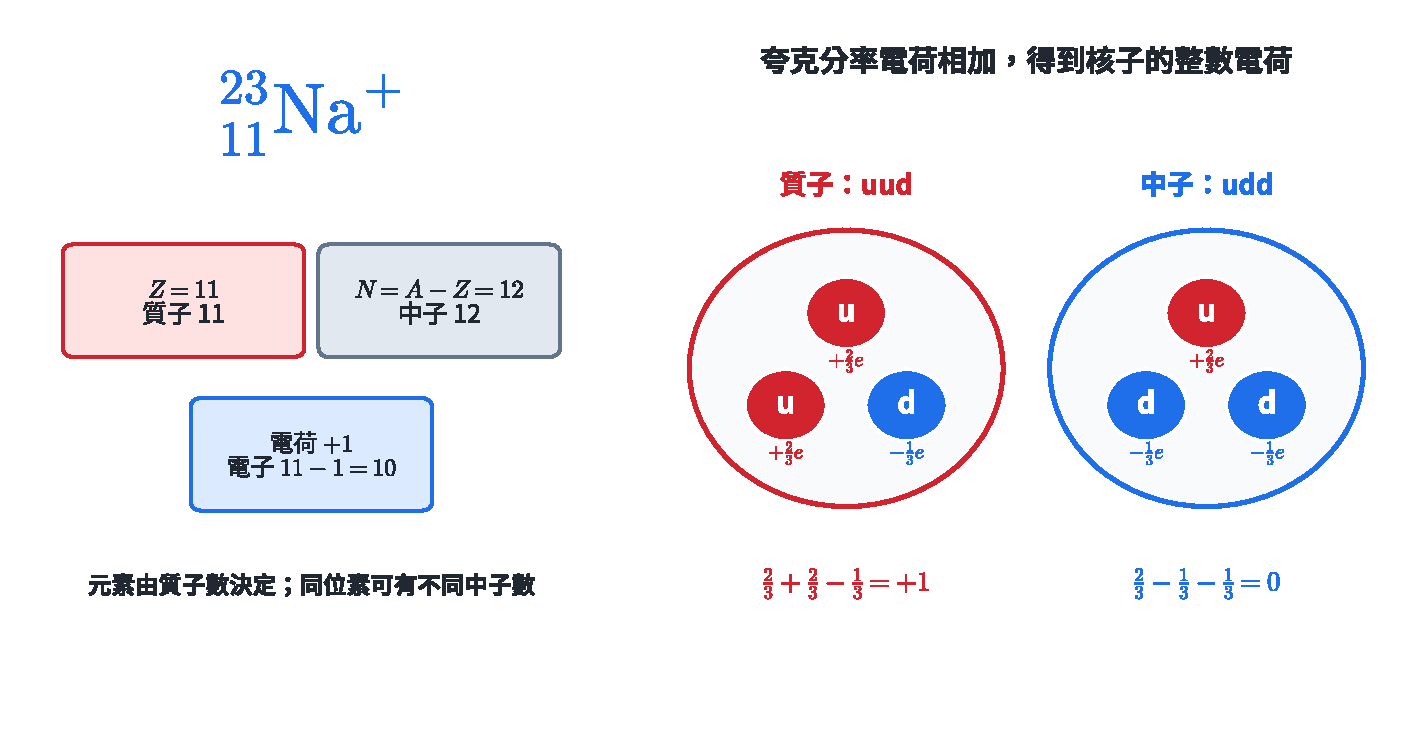
\includegraphics[keepaspectratio,alt={核素記號與夸克組成}]{assets/必物-2-核素記號與夸克組成.pdf}}
\caption{核素記號與夸克組成}
\end{figure}

\[
q(uud)=\frac{2}{3}e+\frac{2}{3}e-\frac{1}{3}e=+e,
\]

\[
q(udd)=\frac{2}{3}e-\frac{1}{3}e-\frac{1}{3}e=0,
\]

\[
q(uuu)=3\left(\frac{2}{3}e\right)=+2e.
\]

\(uud\) 是質子，\(udd\) 是中子；\(uuu\) 的電荷與兩者皆不同。

\subsection{第 9 題}\label{ux7b2c-9-ux984c}

\begin{figure}
\centering
\pandocbounded{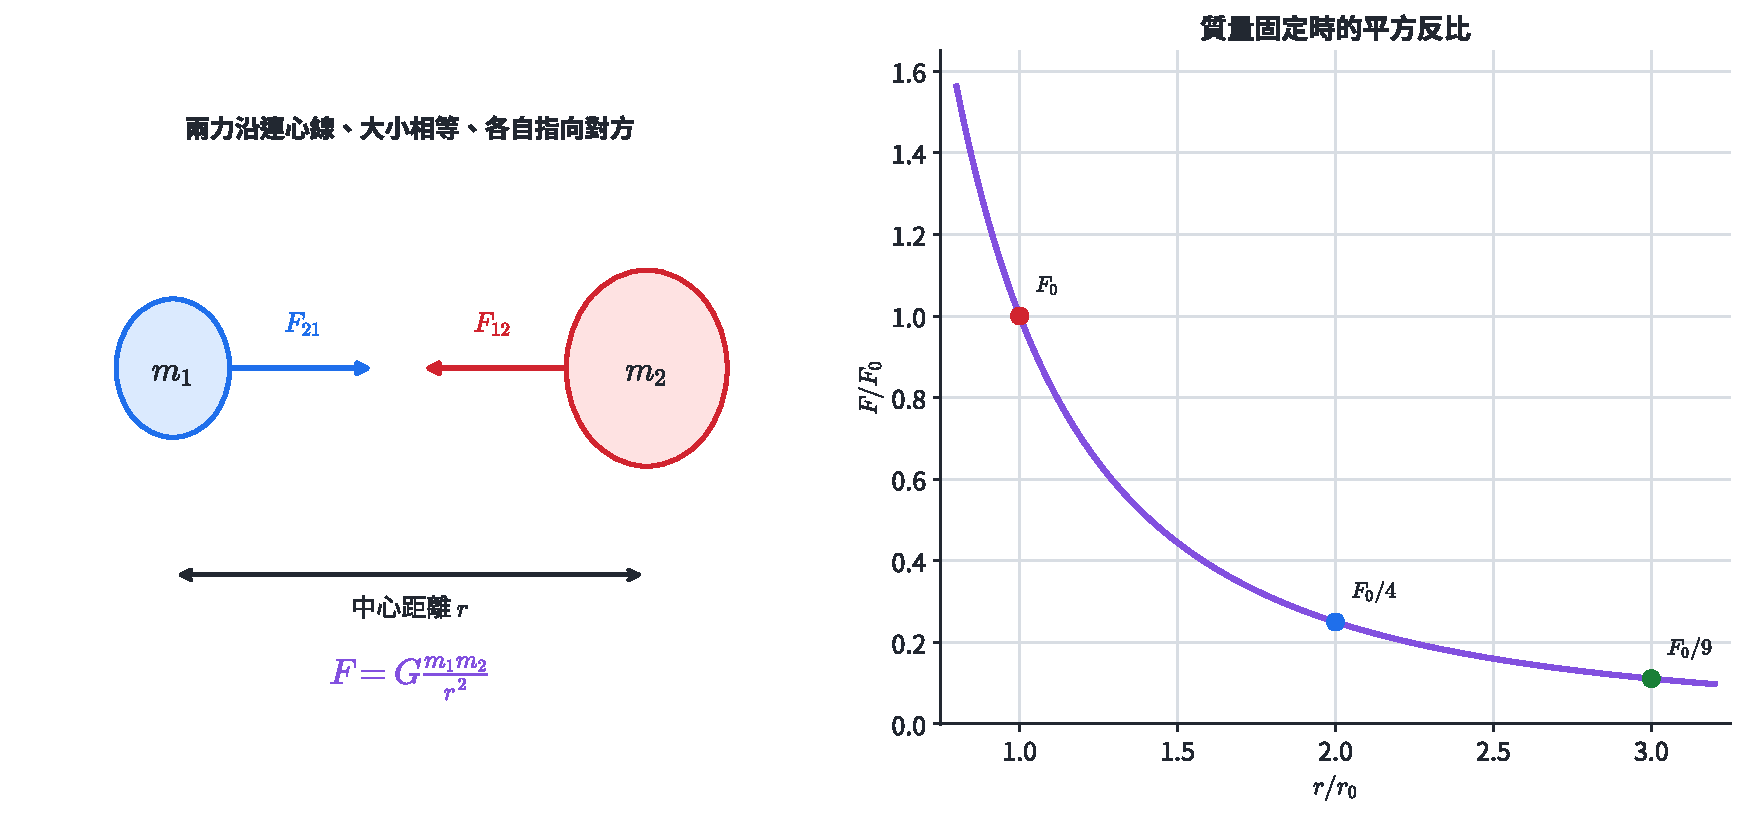
\includegraphics[keepaspectratio,alt={萬有引力與平方反比}]{assets/必物-2-萬有引力與平方反比.pdf}}
\caption{萬有引力與平方反比}
\end{figure}

原狀態的質量乘積是 \(m(2m)\)；新狀態是 \(m(6m)\)，為原來 3 倍。距離變 3 倍，平方反比給 \(1/9\)：

\[
\frac{F'}{F}=3\cdot\frac{1}{9}=\frac{1}{3}.
\]

答案：

\[
F'=\frac{F}{3}.
\]

\subsection{第 10 題}\label{ux7b2c-10-ux984c}

\begin{figure}
\centering
\pandocbounded{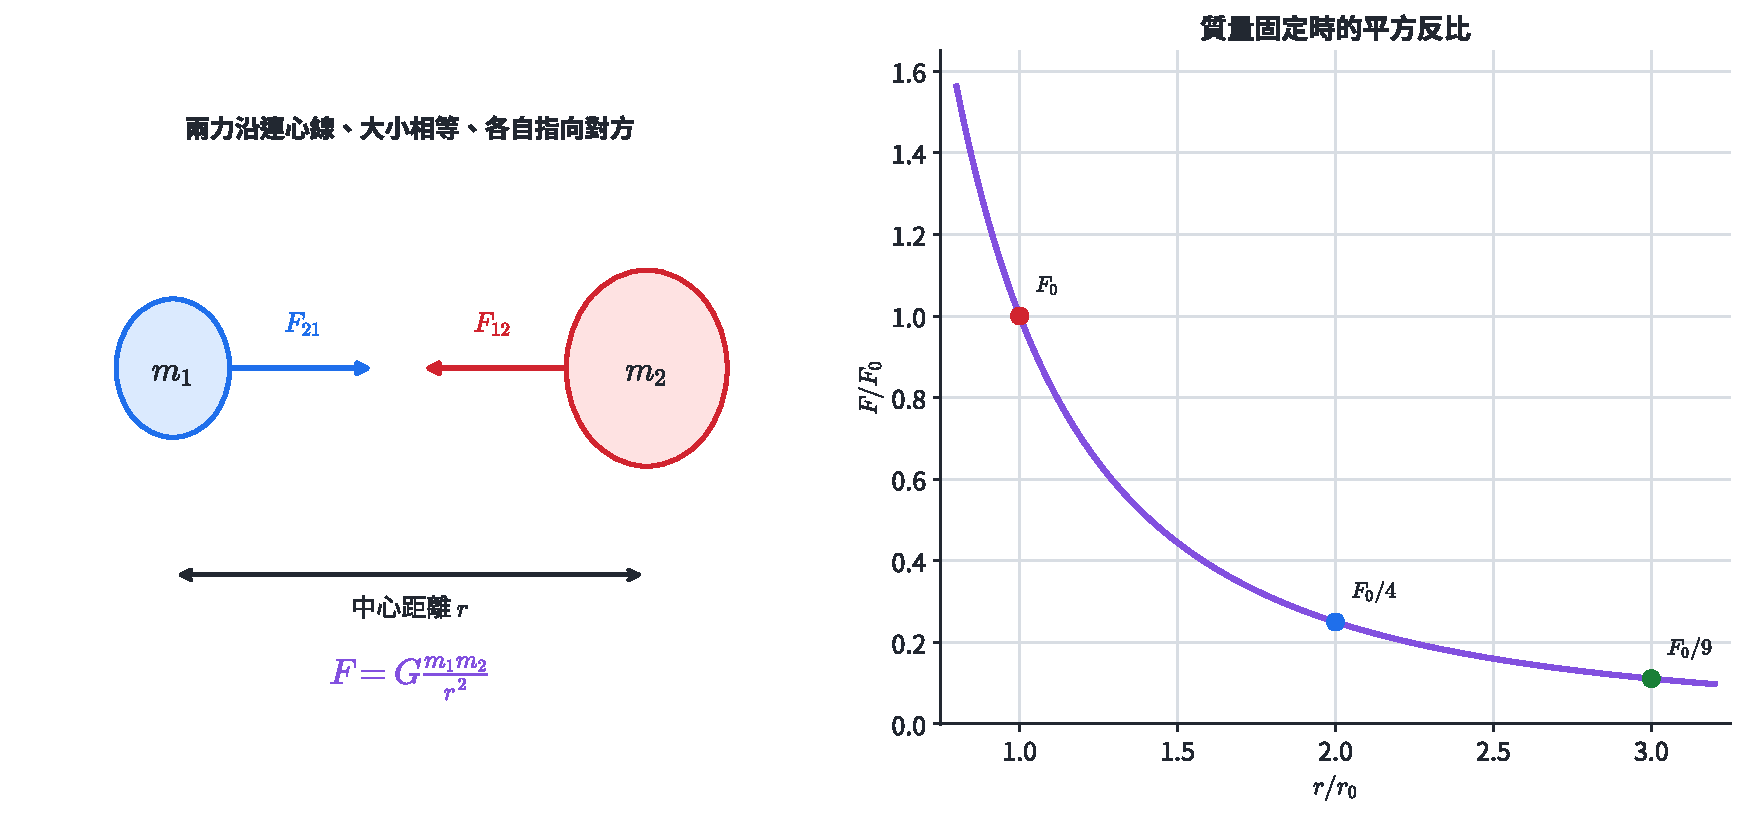
\includegraphics[keepaspectratio,alt={萬有引力與平方反比}]{assets/必物-2-萬有引力與平方反比.pdf}}
\caption{萬有引力與平方反比}
\end{figure}

\[
\frac{g'}{g_\oplus}
=\frac{9M_\oplus}{M_\oplus}
\left(\frac{R_\oplus}{3R_\oplus}\right)^2
=9\cdot\frac{1}{9}=1.
\]

表面重力加速度相同。同一物體的質量是物體本身性質，在兩地相同；重量 \(W=mg\)，因 \(g\) 相同，所以重量也相同。

\subsection{第 11 題}\label{ux7b2c-11-ux984c}

\begin{figure}
\centering
\pandocbounded{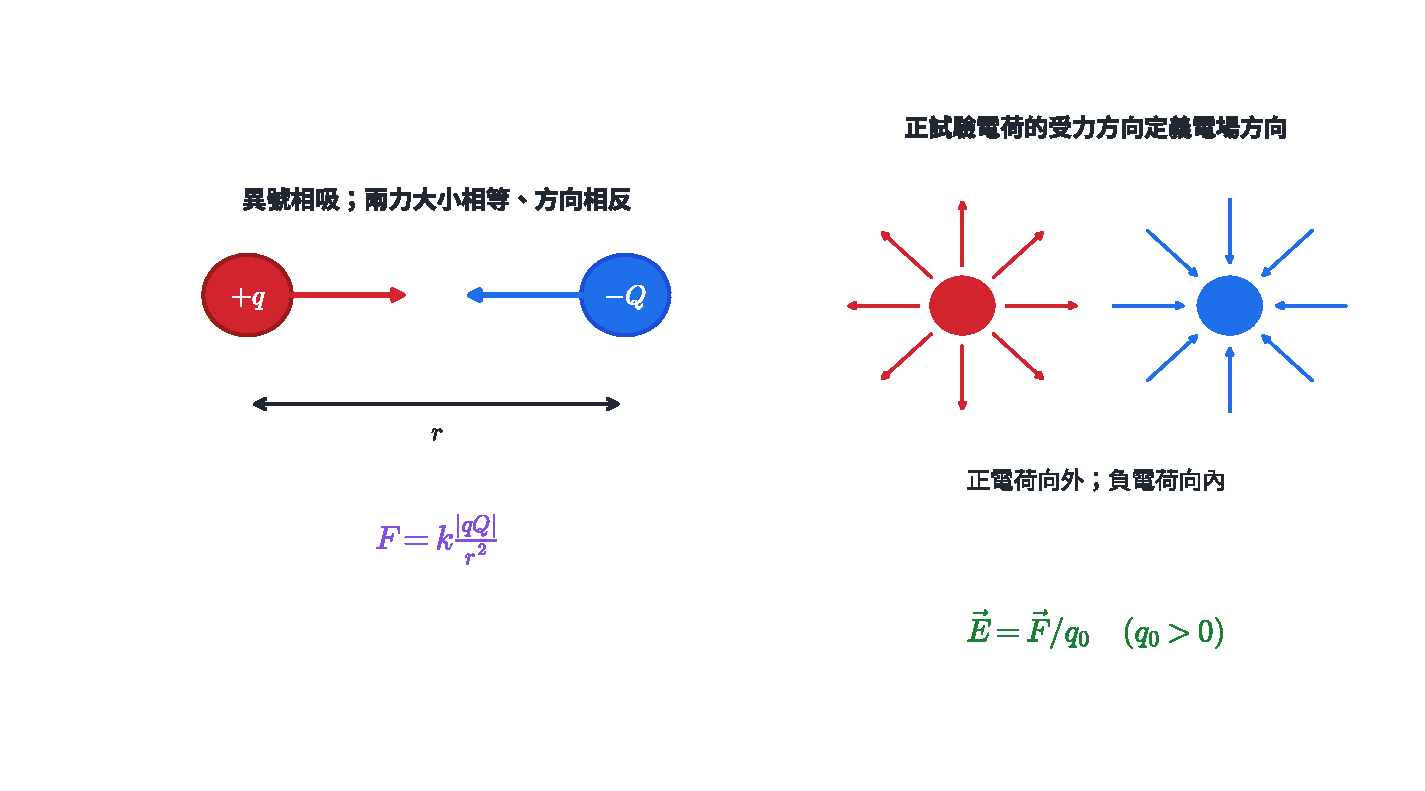
\includegraphics[keepaspectratio,alt={庫侖力與電場線}]{assets/必物-2-庫侖力與電場線.pdf}}
\caption{庫侖力與電場線}
\end{figure}

在中點：

\begin{itemize}
\tightlist
\item
  \(+Q\) 的電場指離正電荷。
\item
  \(-Q\) 的電場指向負電荷。
\end{itemize}

兩者都由 \(+Q\) 指向 \(-Q\)，所以相加。中點距各電荷為 \(a\)：

\[
E=2k\frac{Q}{a^2}.
\]

改變後

\[
E'=2k\frac{2Q}{(2a)^2}
=2k\frac{Q}{a^2}\cdot\frac{1}{2}
=\frac{E}{2}.
\]

方向仍由正電荷指向負電荷。

\subsection{第 12 題}\label{ux7b2c-12-ux984c}

\begin{figure}
\centering
\pandocbounded{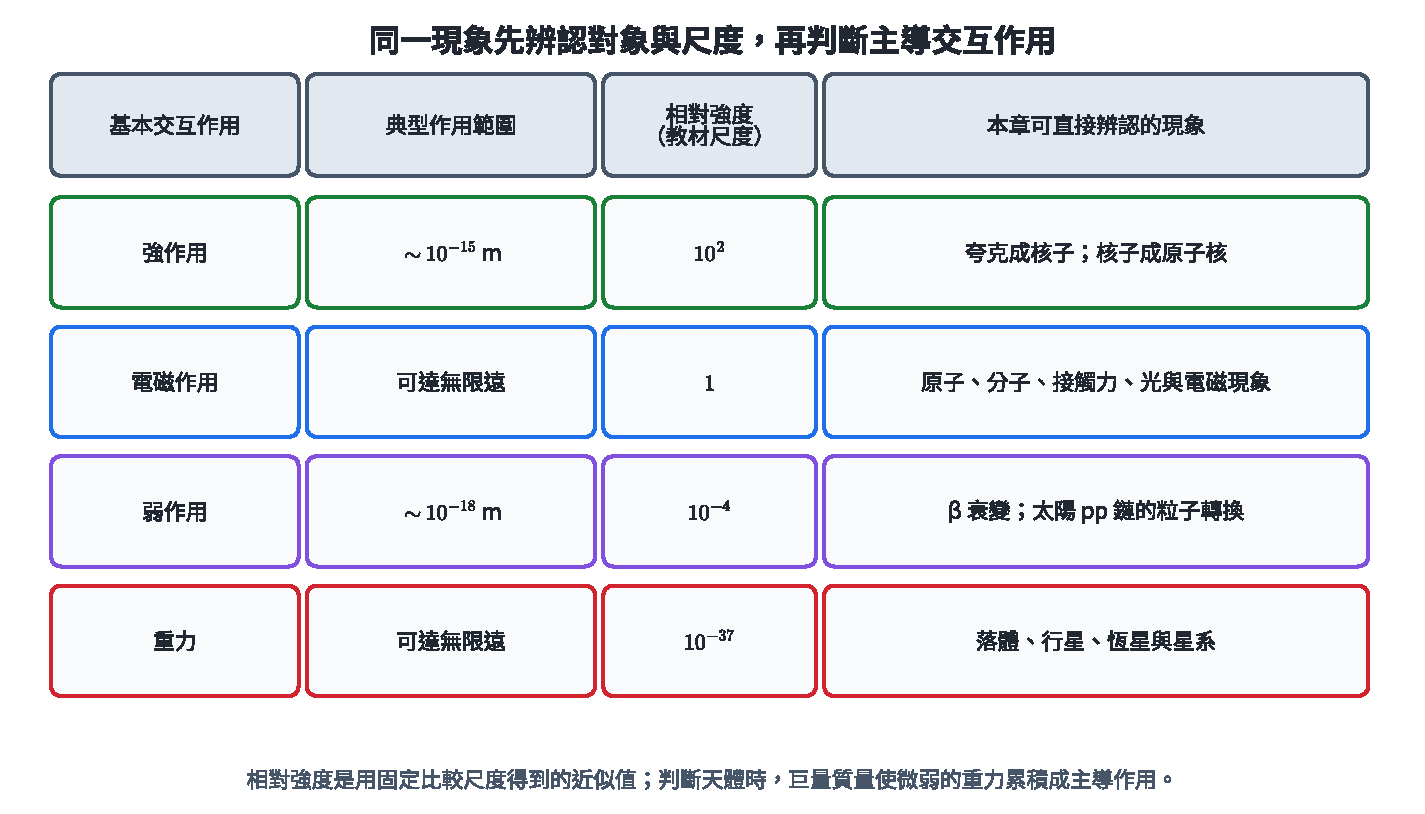
\includegraphics[keepaspectratio,alt={四種基本交互作用尺度圖}]{assets/必物-2-四種基本交互作用尺度圖.pdf}}
\caption{四種基本交互作用尺度圖}
\end{figure}

\begin{itemize}
\tightlist
\item
  甲：磁鐵先使迴紋針磁化，再產生磁吸引，屬電磁作用。
\item
  乙：核子在約 \(10^{-15}\ \mathrm m\) 尺度內受殘餘強作用束縛。
\item
  丙：中子轉為質子、電子與反微中子，屬弱作用。
\item
  丁：地球與太陽都是大質量天體，公轉由萬有引力主導。
\end{itemize}

\subsection{第 13 題}\label{ux7b2c-13-ux984c}

\begin{figure}
\centering
\pandocbounded{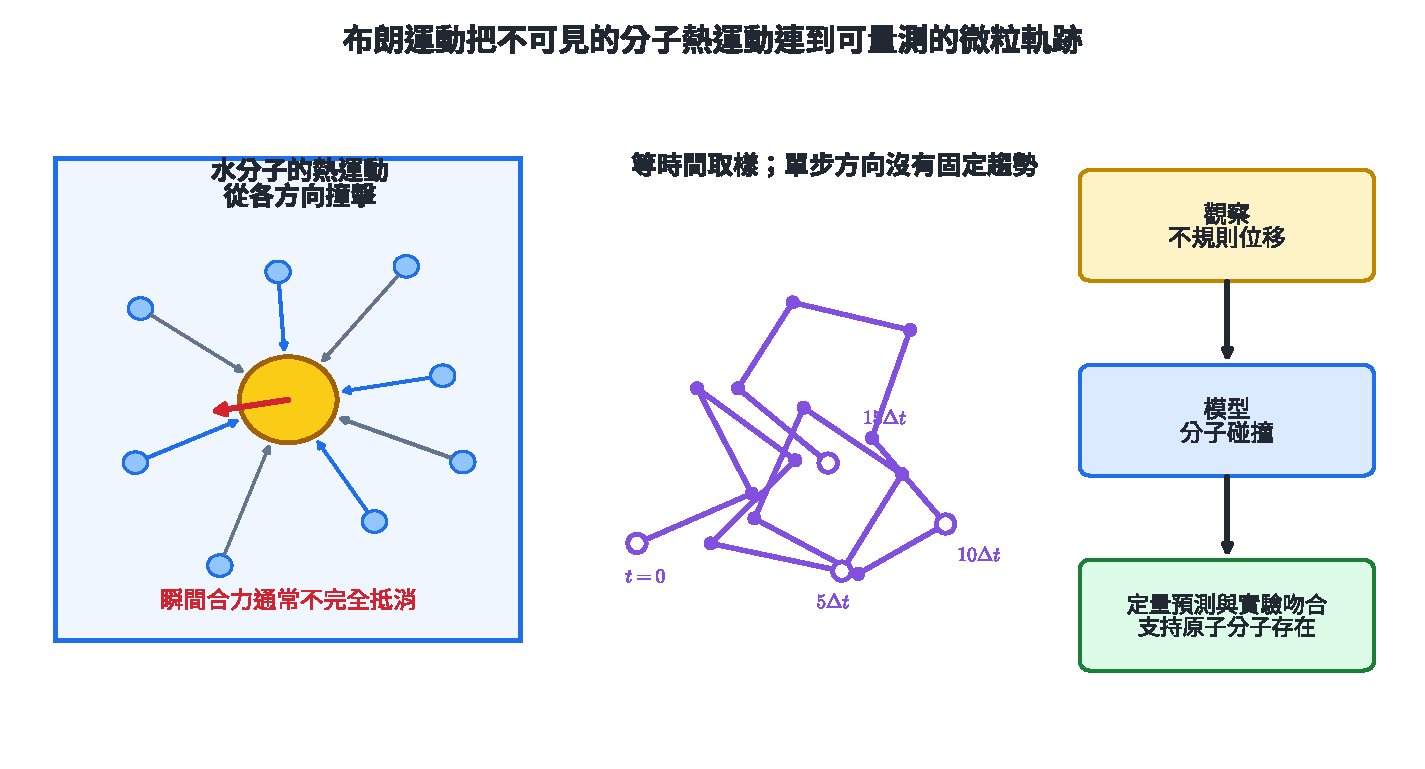
\includegraphics[keepaspectratio,alt={分子碰撞、等時間位置與布朗運動的證據鏈}]{assets/必物-2-原子存在的證據鏈.pdf}}
\caption{分子碰撞、等時間位置與布朗運動的證據鏈}
\end{figure}

\begin{figure}
\centering
\pandocbounded{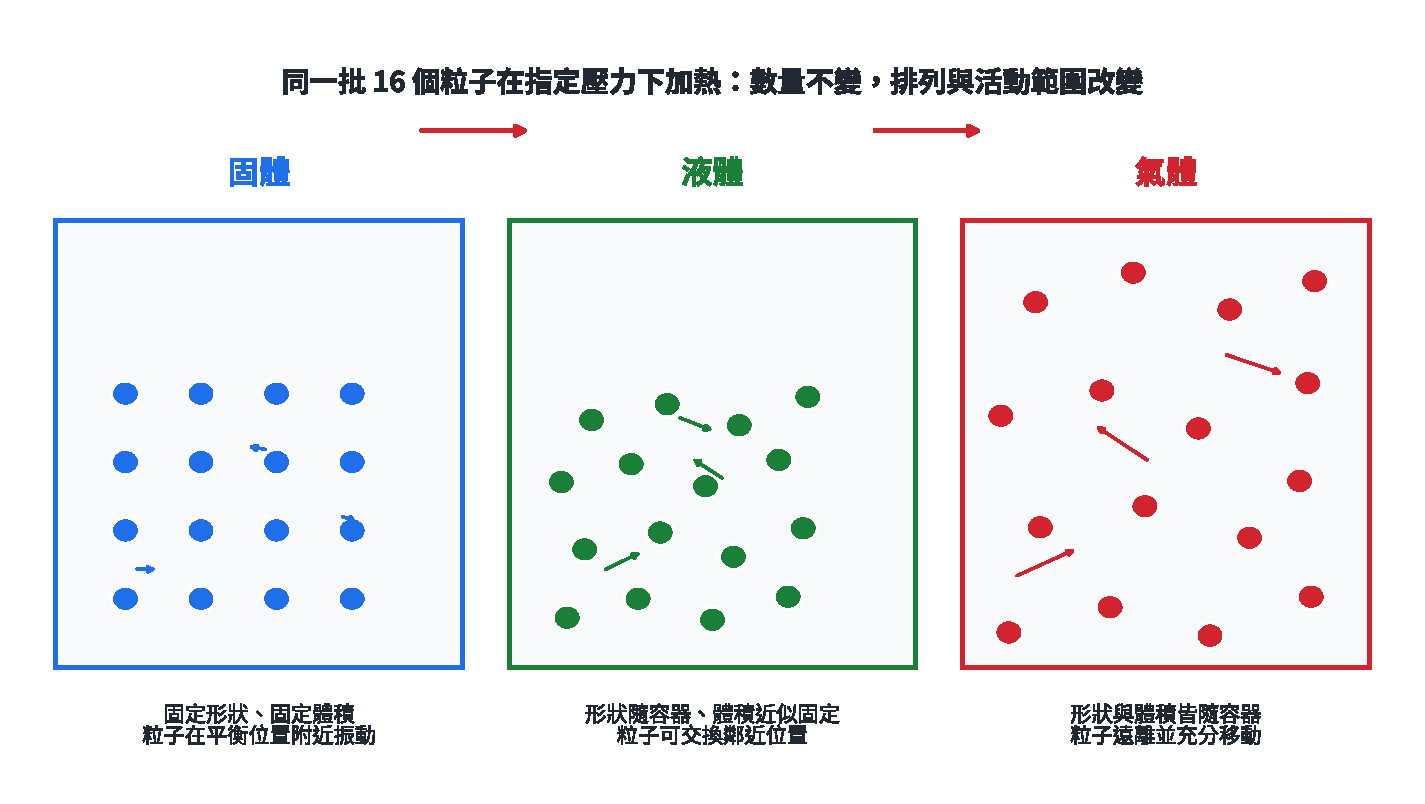
\includegraphics[keepaspectratio,alt={同一批粒子的三態排列、間距與運動}]{assets/必物-2-物質三態的粒子模型.pdf}}
\caption{同一批粒子的三態排列、間距與運動}
\end{figure}

（1）先統一單位：

\[
\frac{80\ \mathrm{nm}}{0.20\ \mathrm{nm}}=400.
\]

奈米粒子直徑約為原子尺度的 400 倍。

（2）觀察是顯微鏡下粒子位置隨時間呈不規則折線；模型是水分子的熱運動造成不平衡碰撞；可控制變因可選水溫、粒徑或液體黏滯性，並比較平均位移平方。

（3）凝固後水分子平均動能降低，鄰近關係形成較穩定結構，粒子主要在局部平衡位置附近振動；材料取得固定形狀與固定體積。

本題連結尺度換算、布朗運動證據與三態粒子模型。

\subsection{第 14 題}\label{ux7b2c-14-ux984c}

\begin{figure}
\centering
\pandocbounded{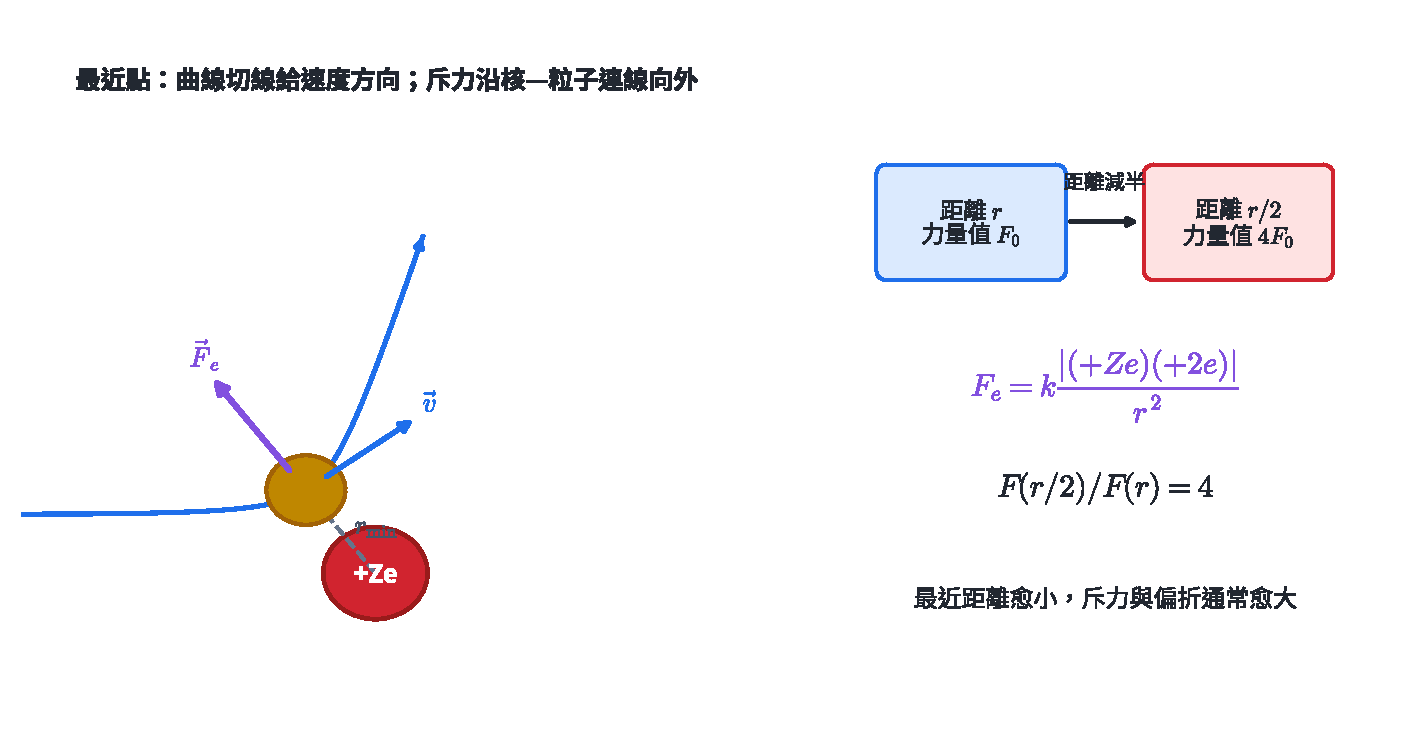
\includegraphics[keepaspectratio,alt={alpha 粒子曲線軌跡、最近點速度與徑向斥力}]{assets/必物-2-alpha粒子最近點受力.pdf}}
\caption{alpha 粒子曲線軌跡、最近點速度與徑向斥力}
\end{figure}

（1）原子核與 \(\alpha\) 粒子都帶正電。\(\alpha\) 粒子位於核上方時，受力沿兩者連線並指向遠離原子核，也就是具有向上分量。

（2）

\[
\frac{F'}{F}
=\left(\frac{r}{r/2}\right)^2
=4.
\]

最近點庫侖力變為 4 倍。

（3）較大的斥力使軌跡彎曲更明顯，偏折角通常增大。極少數大角偏折表示少數粒子非常接近一個小而集中的正電區，支持原子核模型。

\subsection{第 15 題}\label{ux7b2c-15-ux984c}

\begin{figure}
\centering
\pandocbounded{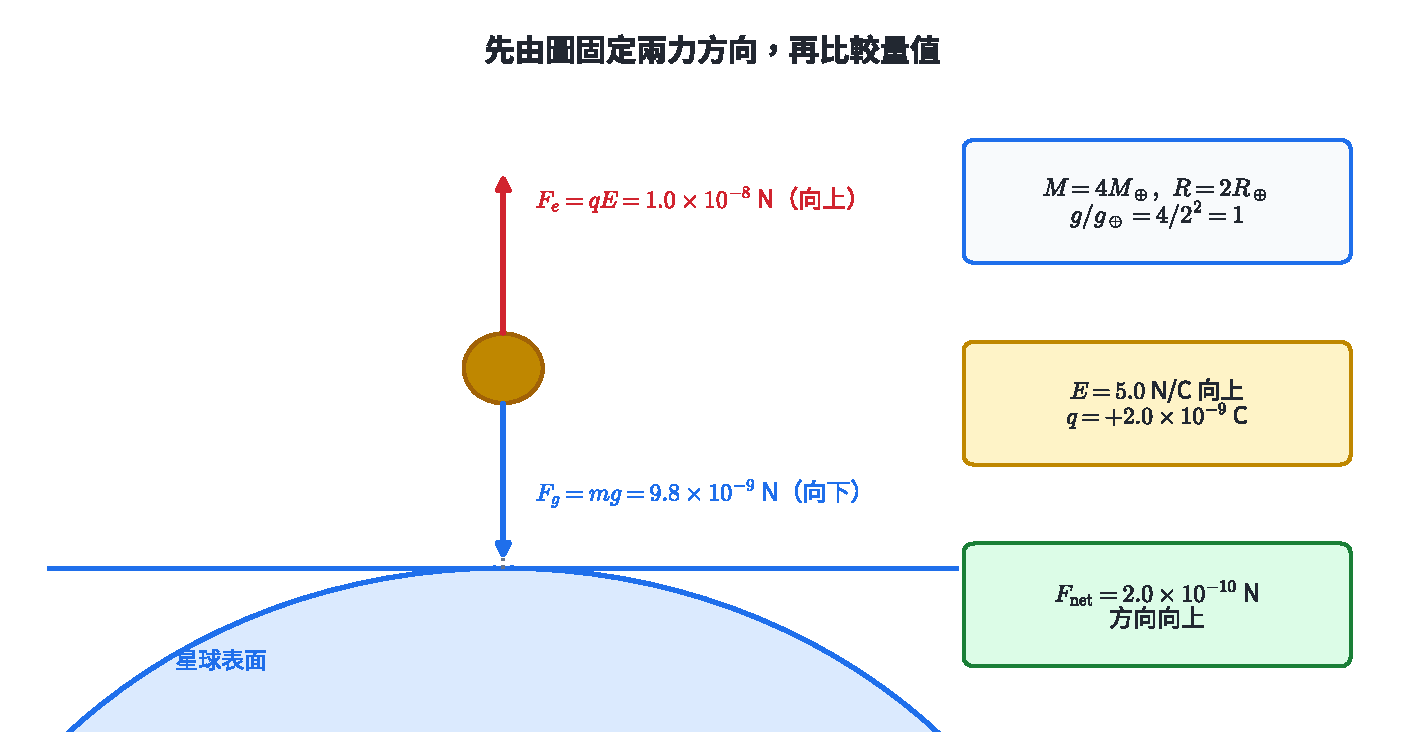
\includegraphics[keepaspectratio,alt={星球表面帶電微粒的受力}]{assets/必物-2-星球表面帶電微粒受力.pdf}}
\caption{星球表面帶電微粒的受力}
\end{figure}

（1）

\[
\frac{g'}{g_\oplus}
=\frac{4}{2^2}=1,
\]

所以

\[
g'=9.8\ \mathrm{m/s^2}.
\]

（2）重力向下：

\[
F_g=mg=(1.0\times10^{-9})(9.8)
=9.8\times10^{-9}\ \mathrm N.
\]

電量為正，電場向上，所以電力向上：

\[
F_e=qE=(2.0\times10^{-9})(5.0)
=1.0\times10^{-8}\ \mathrm N.
\]

（3）

\[
F_e=10.0\times10^{-9}\ \mathrm N
>F_g=9.8\times10^{-9}\ \mathrm N.
\]

電力稍大，淨力為

\[
F_{\text{net}}=2.0\times10^{-10}\ \mathrm N
\]

向上。重力屬重力交互作用；電力屬電磁作用。本題同時使用天體表面 \(g\) 與帶電微粒在電場中的受力。

\subsection{第 16 題}\label{ux7b2c-16-ux984c}

\begin{figure}
\centering
\pandocbounded{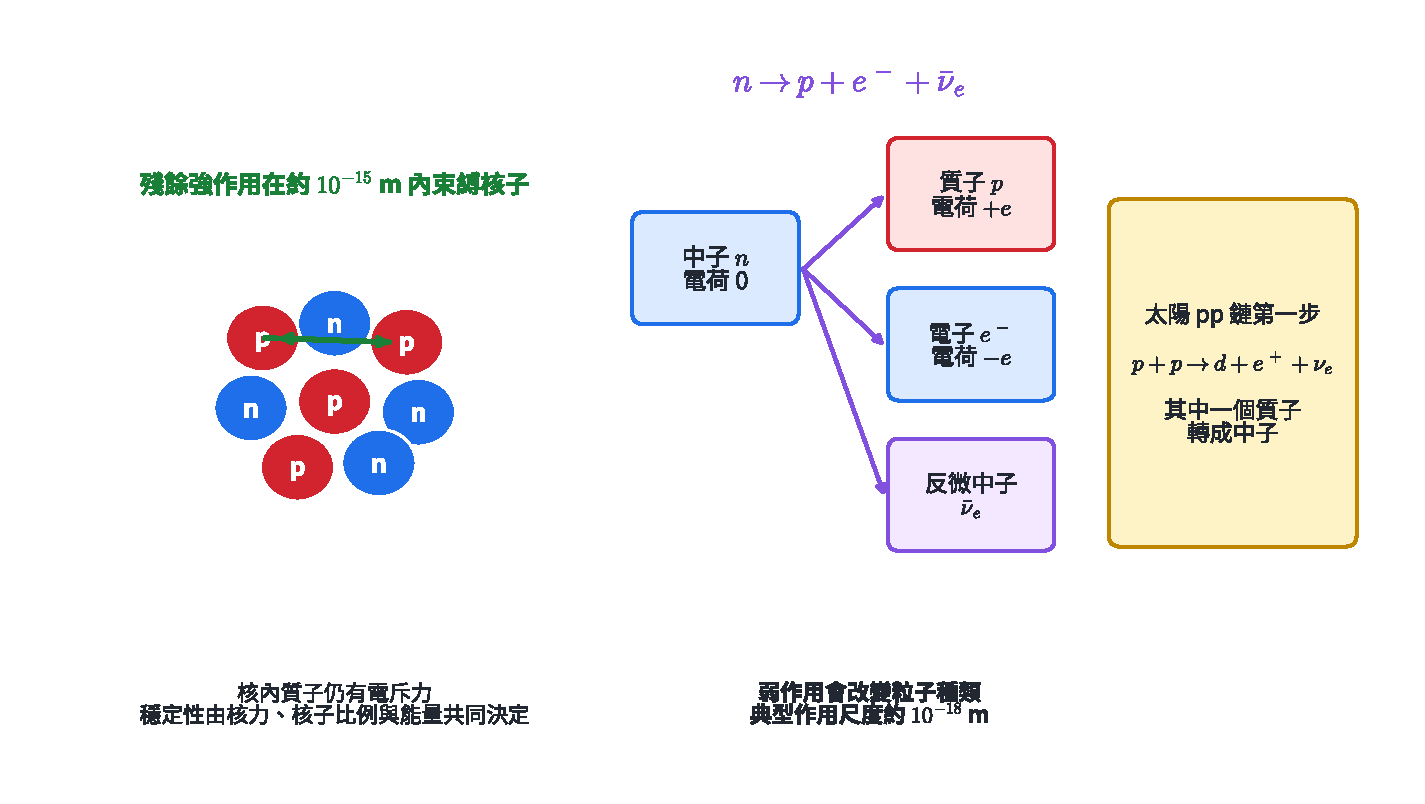
\includegraphics[keepaspectratio,alt={強作用與弱作用}]{assets/必物-2-強作用與弱作用.pdf}}
\caption{強作用與弱作用}
\end{figure}

（1）衰變前：

\[
{}^{14}_{6}\mathrm C:\quad p=6,\quad n=14-6=8.
\]

衰變後：

\[
{}^{14}_{7}\mathrm N:\quad p=7,\quad n=14-7=7.
\]

一個中子轉成一個質子，質量數維持 14。

（2）以 \(e\) 為單位：

\[
\text{左側}=+6,
\]

\[
\text{右側}=+7+(-1)+0=+6.
\]

電荷守恆。

（3）

\begin{itemize}
\tightlist
\item
  中子轉為質子、電子與反微中子：弱作用。
\item
  質子與中子束縛在核內：殘餘強作用。
\item
  核外電子受正原子核吸引：電磁作用。
\end{itemize}

（4）核素記號的 \(Z\) 由 6 變 7、\(A\) 維持 14，直接呈現核內粒子種類改變；夸克層次可把中子的 \(udd\) 轉換連到質子的 \(uud\)；反應機制由弱作用主導，而生成的原子核仍由殘餘強作用束縛。這是一條由符號、粒子組成到交互作用的完整證據鏈。


\end{document}
